\documentclass[12pt, a4paper, twoside]{report}
% encodings and language
\usepackage[T1]{fontenc}
\usepackage[utf8]{inputenc}
\usepackage[spanish, es-noquoting, es-tabla]{babel}
%graphics and colors
\usepackage{graphicx}
\usepackage{float}
\usepackage{color}
\graphicspath{ {figures/} }
%math symbols and fonts
\usepackage{amsmath, amssymb, amsfonts}
% miscellaneous
\usepackage{authblk}
\usepackage{hyperref}
\usepackage{caption}
\usepackage{subcaption}
\usepackage{booktabs}
\usepackage{multirow}
\usepackage[bottom]{footmisc}

% code coloring
\usepackage[procnames]{listings}
\definecolor{keywords}{RGB}{255,0,90}
\definecolor{comments}{RGB}{0,0,113}
\definecolor{red}{RGB}{160,0,0}
\definecolor{green}{RGB}{0,150,0}
\lstset{
		language=Python, 
        basicstyle=\ttfamily\small, 
        keywordstyle=\color{keywords},
        commentstyle=\color{comments},
        stringstyle=\color{red},
        showstringspaces=false,
        identifierstyle=\color{green},
        procnamekeys={def,class},
    	frame=single,
    	breaklines=true,
    	postbreak=\raisebox{0ex}[0ex][0ex]{\ensuremath{\color{red}\hookrightarrow\space}}
}

% page geometry
\usepackage[a4paper,width=170mm,top=25mm,bottom=25mm,bindingoffset=6mm]{geometry}
\setlength{\headheight}{15pt}
\linespread{1.5}
\raggedbottom

%fancy headers
\usepackage{fancyhdr}
\pagestyle{fancy}

\newcommand\doubleRule{\toprule\toprule}
\newcommand\doublerule{\toprule\specialrule{\heavyrulewidth}{\doublerulesep}{0.95em}}

\fancyhead{}
%\fancyhead[RO,LE]{\leftmark}
\fancyhead[LO,RE]{\rightmark}
\fancyfoot{}
\fancyfoot[CE,CO]{\thepage}

% bibliography
\usepackage{biblatex}
\bibliography{chapters/referencias}


\begin{document}
\begin{titlepage}
    \begin{center}
        \vspace*{1cm}
        
        \Large{\textbf{Caracterización acústica de un acuario para estudios comportamentales}}
        
        \vspace{0.5cm}
        \large{Caracterización y modificación de los campos acústicos de una pecera pequeña}
        
        \vfill
        
        Informe final de Laboratorio 6 y 7.
        
        \vspace{0.8cm}
        
        
\includegraphics[width=0.4\textwidth]{figures/logodf}
        
        Departamento de Física\\
        Facultad de Ciencias Exactas y Naturales\\
        Universidad de Buenos Aires\\
        Diciembre de 2016
        
    \end{center}
\end{titlepage}
\newpage
\begin{titlepage}
	\begin{flushleft}
	    \vspace{1.5cm}
        
        \textbf{Alumno}: Juan Ignacio Beiroa, LU 559/10, \href{mailto:jbeiroa@gmail.com}{jbeiroa@gmail.com}.
        
        \vspace{1.5cm}
        
        \textbf{Lugar de trabajo:} Laboratorio de Fisiología y Biología Molecular, FCEyN.
        
        \vspace{2.5cm}
        
        \textbf{Directora:} Violeta Medan, \href{mailto:violetamedan@gmail.com}{violetamedan@gmail.com}.
        
        \textbf{Codirector:} Manuel Eguía, \href{mailto:eguiamc@gmail.com}{eguiamc@gmail.com}, \href{http://www.lapso.org/}{Laboratorio de Acústica y Percepción Sonora (UNQ)}.

	\end{flushleft}
	\vfill
	\begin{center}
		\textbf{Violeta Medan} \hfill \textbf{Juan Ignacio Beiroa} \hfill \textbf{Manuel Eguía}
	\end{center}
\end{titlepage}
\pagenumbering{roman}
\chapter*{Motivaciones y objetivos}
En todos los peces óseos, existe un circuito neuronal que controla una respuesta de escape o sobresalto. En forma muy simplificada, este circuito, consta de tres elementos: aferencias (entradas) sensoriales que colectan información del medio; una interneurona, la célula Mauthner, que funciona como elemento integrador de las entradas sensoriales y que gatilla (mediante el disparo de un potencial de acción) la contracción masiva de la musculatura que permite la respuesta de escape; mediada por neuronas motoras. Este reflejo de escape puede ser causado por distintos estímulos sensoriales, siendo los acústicos y visuales los más estudiados. En el caso de peces de descarga eléctrica débil como \emph{Gymnotus omarorum}, también modula la descarga del órgano eléctrico (DOE).

Los peces de descarga eléctrica débil emiten en forma constante un campo eléctrico pulsado que sufre deformaciones al atravesar un medio de conductancia heterogénea. Los animales son capaces de detectar su propio campo eléctrico y por lo tanto utilizan esas descargas como parte de un sistema electrosensorial que les permite formar una ``imagen eléctrica'' de su entorno. El experimento típico para evaluar la respuesta de escape o sobresalto consiste en utilizar algún estímulo acústico o visual que sobresalte al animal y gatille su respuesta mientras se filma el comportamiento del pez y se registra la DOE. Sin embargo, este experimento aún no se ha realizado en peces eléctricos.

En la mayoría de los casos estudiados en peces donde hay una respuesta motora clara, ésta es direccional y propulsa al animal en dirección contraria a la del estímulo. En los peces eléctricos la respuesta de escape o novedad frente a estímulos sonoros no ha sido estudiada y no se ha determinado si hay correlatos entre la modulación de la DOE y respuestas motoras (de escape).

En los experimentos comportamentales es de suma importancia la caracterización física de los estímulos y los dispositivos experimentales utilizados. La primera permite conocer a qué responde el animal y la segunda recrear condiciones controlables y repetitivas que asemejen a aquellas encontradas en los habitats naturales. Desde el punto de vista biológico existe otra razón para la caracterización física, y es que los animales \emph{integran distintas aferencias sensoriales} y en ocasiones es difícil realizar excitaciones que no sean multimodales. En el caso de peces eléctricos, por ejemplo, una estimulación acústica con un parlante sumergido en la pecera conlleva también la posible estimulación causada por la corriente enviada al parlante (y su consiguiente campo magnético). De esta manera, lo que a simple vista es sólo un estímulo sonoro son en realidad tres: el campo acústico de presiones, el campo de velocidades debido a la onda acústica y los campos electromagnéticos del parlante.

En el caso de los estímulos acústicos las propiedades del acuario dificultan el control del experimento. Por un lado, la diferencia de velocidades de propagación entre el agua y el aire hace que todas las interfaces se comporten como espejos acústicos casi ideales, con lo cual una sola fuente de sonido dentro del acuario podría generar suficientes fuentes imágenes para que el sonido parezca provenir de todas las direcciones posibles. 

Como paso previo a futuros estudios de integración multimodal, se ha realizado una caracterización acústica de una pecera para estudios comportamentales. Los objetivos principales del proyecto contemplaban la caracterización a partir mediciones de la respuesta impulso del acuario, el armado del setup experimental para los estudios comportamentales y la posible implementación de un sistema de control activo de ecos. De estos tres, sólo los primeros dos pudieron llevarse a cabo completamente.

\chapter*{Resumen}

Se construyó y caracterizó acústicamente una pecera para realizar estudios comportamentales en peces. El objetivo de dicha caracterización fué determinar la direccionalidad de los campos de presión que se establecen en el acuario al emitir sonidos con un parlante, siendo de particular interés averigüar si hay excitación de modos normales. Esto último se logró mediante grabaciones y procesamientos acordes de señales de prueba que permiten obtener la respuesta impulso de la pecera. Se observaron modos en casi todo el rango de frecuencias estudiadas.

Las mediciones realizadas fueron comparadas con modelos computacionales que incluyen ciertas aproximaciones en las condiciones de borde de la pecera. De los modos encontrados, los de frecuencias mayores a 6kHz corresponden a la pecera comportándose como una guía de ondas, mientras que los de frecuencias más bajas se deben a la interacción del agua con los vidrios y el aire en la superficie libre. Estos últimos aparecen en frecuencias de relevancia biológica y presentan campos uniformes y de direccionalidad clara sólo en una mitad de la pecera, la cual se utilizó para los estudios comportamentales.

La demarcación de la zona experimental se realizó utilizando goma de neoprene, la cual baja la intensidad de todos los modos encontrados y absorve completametamente los de altas frecuencias.

Los estudios compotamentales se hicieron en peces eléctricos se hicieron mediante un programa de adquisición y control desarrollado en el laboratorio. Los resultados muestran que el animal responde ante el estímulo aumentando la frecuencia de la DOE, aunque no siempre hay una respuesta motora.


\tableofcontents

\pagenumbering{arabic}

\chapter{Introducción} 

\section{Caracterización acústica}

\subsection{Planteo físico y modelado por elementos finitos}

El experimento típico que se desea realizar consiste en estimular una respuesta de escape o sobresalto utilizando como fuente un parlante sumergido en la pecera. Una caracterización total de la acústica consistiría en:
\begin{itemize}
	\item La caracterización del parlante como emisor de sonido, principalmente la determinación de la direccionalidad de emisión.
	\item La caracterización de los campos acústicos dentro de la pecera, de presiones y de velocidades del medio (agua).
\end{itemize}
La caracterización del parlante requiere medir patrones de emisión en condiciones de campo libre donde los bordes de la pecera (o pileta) se encuentren a varias longitudes de onda del parlante; impracticable en una pecera de laboratorio. Para el estudio de los campos acústicos se requiere de hidrófonos (medidores de presión) y de un acelerómetro sumergible de alta presición. Inicialmente se planteó caracterizar ambos campos, pero el alto costo presupuestado para el acelerómetro (US\$5000) sólo permitió la caracterización del campo de presiones.

La onda sonora está completamente determinada por la ecuación de ondas de Helmholtz
\begin{equation}
	\nabla^2p(\vec{r})\,+\,\left(\frac{2\pi}{\lambda}\right)^2p(\vec{r})\,=\,0,
	\label{eq:helmholtz}
\end{equation}
la cual permite conocer el campo de presiones $p(\vec{r})$ para cualquier coordenada $\vec{r}$ dada la longitud de onda $\lambda$ (para aliviar la notación se han omitido las dependencias temporales en todas las fórmulas, y en lo siguiente también se omitirán las espaciales). Para completar la determinación del problema, se debe tener en cuenta que las partículas del medio se moverán siempre que se imponga un campo de presiones de gradiente no nulo. Las velocidades pueden obtenerse mediante aproximaciones de la ecuación de Navier-Stokes y la adición de una ecuación de estado:

\begin{align}
	\rho\,\frac{\partial\vec{u}}{\partial t}\,=\,-\vec{\nabla}p,
	\label{eq:stokes}\\
	p\,=\,c^2\,\rho '.
	\label{eq:fluidos}
\end{align}

Aquí, $\vec{u}$ es el campo de velocidades y $\rho$ la densidad estática del medio ($\approx$ 1g/m\textsuperscript{3} para el agua), $c$ es la velocidad de propagación del sonido en el medio ($\approx$ 1500m/s en agua) y $\rho'$ la densidad acústica.

La resolución de las ecuaciones \ref{eq:helmholtz}, \ref{eq:stokes} y \ref{eq:fluidos} no puede obtenerse en forma analítica y se debe recurrir a aproximaciones o métodos computacionales. En la bibliografía suelen encontrarse dos aproximaciones, la primera concierne a la ecuación de Helmholtz \ref{eq:helmholtz} y la segunda a las condiciones de borde.

En el rango de frecuencias de 20Hz hasta 20kHz las longitudes de onda en agua son de 0,75m hasta 75m, siendo los rangos de longitudes más grandes (menores frecuencias) los de mayor relevancia biológica. Esto implica que, en el caso más general, la longitud de onda es siempre mucho mayor que las medidas del acuario experimental (suelen ser del orden del metro) y la ecuación de Helmholtz \ref{eq:helmholtz} puede ser aproximada por la ecuación de Laplace:

\begin{equation}
	\vec{\nabla}p=0.
	\label{eq:laplace}
\end{equation} 

En cuanto a las condiciones de borde, en principio debería plantearse un cambio de medio en todas las superficies, agua-vidrio-aire para las paredes y agua-aire para la superficie libre. Sin embargo, los vidrios y plásticos utilizados en la construcción de peceras se doblan fácilmente con las presiones acústicas, y aún cerca de las paredes existe movimiento de partículas. Esto quiere decir que, a primer orden, el acuario se comporta como un bloque de agua aislado con condiciones de bordes suave (pressure release). Si la fuente de sonido está dentro del agua, la presión se anula en todas las superficies pero los campos de velocidades no. Estas condiciones, opuestas a las utilizadas generalmente en aire (bordes duros, velocidad nula en interfaces) son las que le dan complejidad al problema.

Utilizando las aproximaciones discutidas, se pueden derivar de la ecuación de Laplace \ref{eq:laplace} las frecuencias de los modos resonantes \emph{sólo del agua}. Esto es, aquellos modos que no se deban a la interacción con el material del acuario. Dichas frecuencias están dadas por la ecuación [1]
\begin{equation}
	f_{lmn}\,=\,\frac{c}{2}\sqrt{\frac{l}{L^2_x}\,+\,\frac{l}{L^2_y}\,+\,\frac{l}{L^2_z}},
	\label{eq:resonancias}
\end{equation}
donde $l$, $m$ y $n$ se refieren al número de modo y $L_x$, $L_y$ y $L_z$ son las dimensiones del acuario.

La mayoría de los estudios bibliográficos utilizan las aproximaciones discutidas y no tienen en cuenta la interacción del agua con el aire ni el vidrio [2, 3]. Con el objetivo de realizar un estudio más completo se recurrió al análisis por elementos finitos mediante el software COMSOL Multiphysics\textregistered 5.2.

Se programó un modelo del acuario en COMSOL y se exploraron distintas condiciones de borde, rodeando a la pecera con una capa perfectamente acoplada (perfectly matched layer) que simula al aire circundante.  Modelar las interfases como borde suave da lugar a resultados que concuerdan con las aproximaciones discutidas y los resultados que se obtienen de las ecuaciones \ref{eq:laplace} y \ref{eq:resonancias}. Se decidió, guiado en parte por resultados obtenidos, modelar sólo las interfases agua-vidrio como bordes suave y dejar la superficie libre del acuario como una discontinuidad en el medio de propagación (agua-aire). Con esas condiciones de borde, el programa calcula en forma numérica los campos de presiones en toda la pecera para distintas frecuencias en el rango de 400Hz hasta 10kHz. Como fuente de sonido se utiliza un emisor de ondas planas de geometría cilíndrica; ubicado en el mismo lugar donde se coloca el parlante en los experimentos.

\subsection{Caracterización mediante respuestas impulso}
\label{sec:introsweeps}

Para comparar el modelado numérico con la realidad del experimento, debe medirse la respuesta del acuario a todas las frecuencias utilizadas y en todos los puntos calculados. Este método de caracterización implica una cantidad de tiempo significativa para las condiciones experimentales trabajadas, pero se pueden obtener relaciones señal-ruido enormes debido a la concentración de energía en una sóla frecuencia. Sin embargo, existen otras complicaciones: en la práctica, todos los amplificadores y el parlante utilizado producen distorsión armónica. Esto quiere decir que al querer emitir un tono puro de frecuencia definida, inevitablemente se emitirán también tonos de frecuencias más altas. Para analizar estas mediciones se debe filtrar y rectificar la frecuencia fundamental o procesar la señal mediante transformadas de Fourier y obtener la fundamental a partir del espectro. Ambos métodos son complicados en cuanto al setup a utilizar: el primero requiere de filtros pasa banda de alta precisión y selectividad, mientras que el segundo sólo es posible mediante la generación digital de la señal y la sincronización del conversor DA del emisor y el AD del receptor. 

Es por eso que, en general, siempre es preferible recurrir a la determinación de la \emph{respuesta impulso} (RI). La RI de un sistema acústico es la respuesta del sistema a una pequeña perturbación de duración breve (un impulso, teóricamente una delta de Dirac). En acústica y procesamiento de señales la RI es una función temporal, $h(t)$, que al ser convolucionada con una perturbación cualquiera, $x(t)$, da como resultado la respuesta $y(t)$ del sistema al estímulo:

\begin{equation}
	y(t)\,=\,h(t)\,\otimes\,x(t).
\end{equation}

Para sistemas lineales y temporalmente invariantes, la transformada de la respuesta impulso es la función transferencia del sistema en el espacio de frecuencias. Por esta razón, si se logra medir y calcular la RI  del sistema, el mismo quedará completamente determinado.

El método generalmente elegido consiste en excitar al sistema con un barrido en frecuencias (señal de prueba) y obtener la RI mediante una deconvolución aperiódica con un filtro acorde (filtro inverso). En el espacio temporal, la señal de prueba se define como
\begin{equation}
	x(t)\,=\,\sin
	\left\lbrace
	\frac{w_1\,T}{\ln \left(\frac{\omega_2}{\omega_1}\right)}\,
	\left[\exp 
			\left(\frac{t}{T}\ln \left(\frac{\omega_2}{\omega_1}\right)
	\right)\,-\,1\right]
	\right\rbrace,
\end{equation}
y es un barrido que empieza a la frecuencia angular $\omega_1$, y termina a la frecuencia $\omega_2$ después de $T$ segundos. En la práctica, la señal de prueba se genera programando el espectro en el espacio de las frecuencias con un retardo de grupo\footnote{El retardo de grupo es el retardo temporal de la envolvente de la señal, \emph{no es un retardo de fase.}} que incremente en forma logarítmica. Las formulaciones pertinentes a la generación del barrido pueden encontrarse en [4] y una introducción larga y amena al método en [5]. Un espectrograma de una señal de prueba puede observarse en la figura \ref{fig:testsweep}.

\begin{figure}[H]
	\centering
		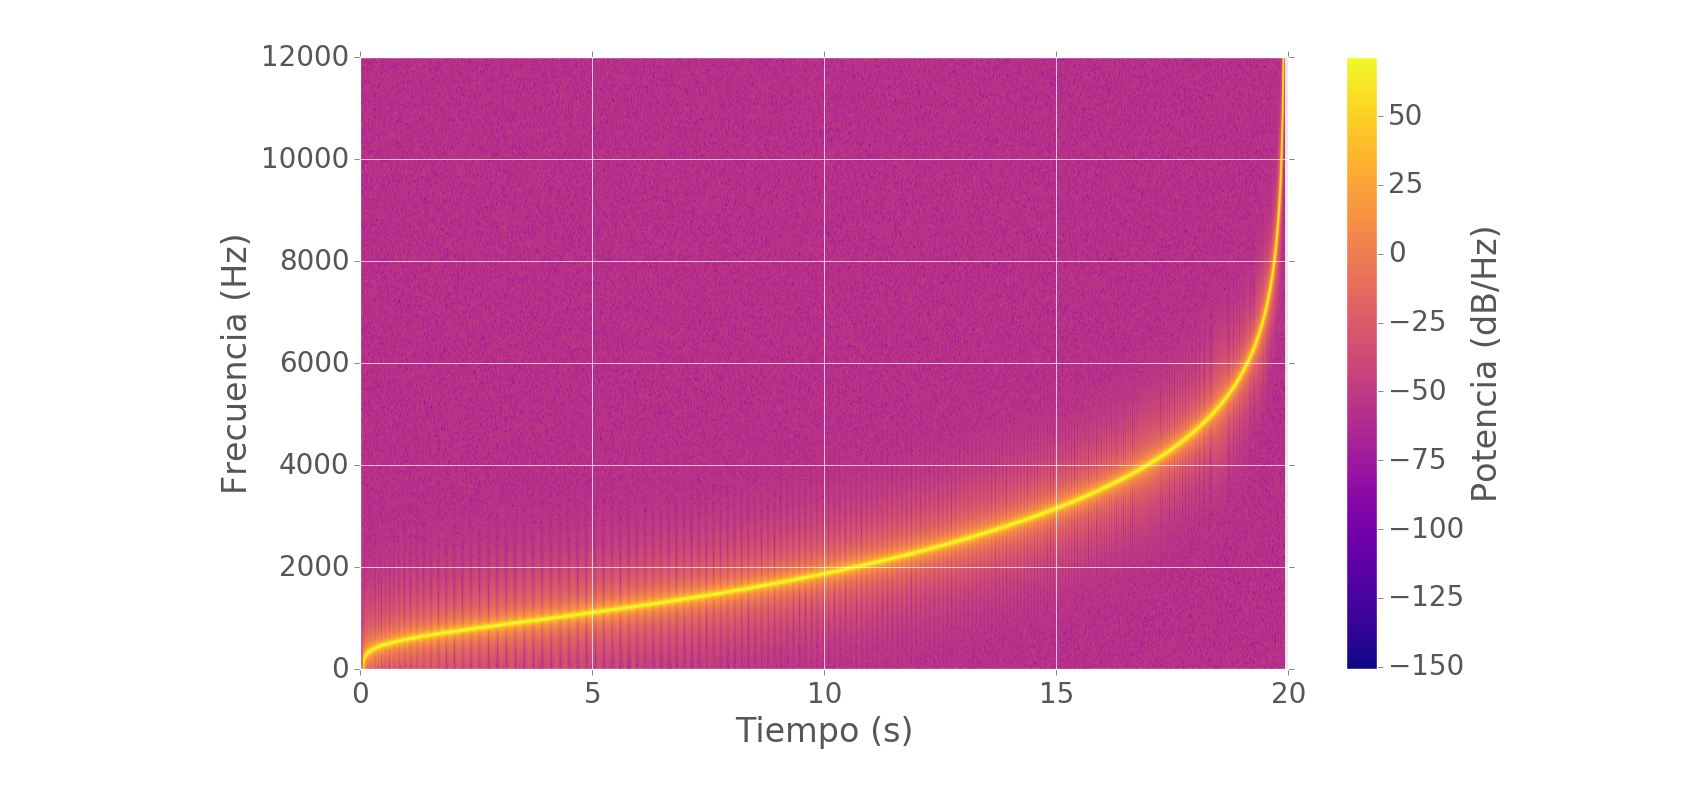
\includegraphics[scale=.43]{testsweep.png}
		\caption{Señal de prueba generada en el espacio de frecuencias. La linea amarilla representa una función senoidal cuya frecuencia varía en forma exponencial en función del tiempo. La frecuencia sube rápidamente desde 0Hz hasta 400Hz, donde inicia el barrido exponencial hasta 10kHz (luego sube rápidamente hasta la mitad de la frecuencia de muestreo con la que se generó la señal de prueba).}
	\label{fig:testsweep}
\end{figure}

Usualmente, como se muestra en la figura \ref{fig:testrec}, la grabación de la señal de prueba traerá consigo distorsiones armónicas (sobretonos de la señal original). La gran ventaja del método frente a otros existentes es que, si la distorisón armónica no es demasiado grande, se puede separar completamente la RI (\emph{respuesta lineal} del medio) de la distorsión armónica (producida por no linealidades en amplificadores y parlantes). 

\begin{figure}[H]
	\centering
		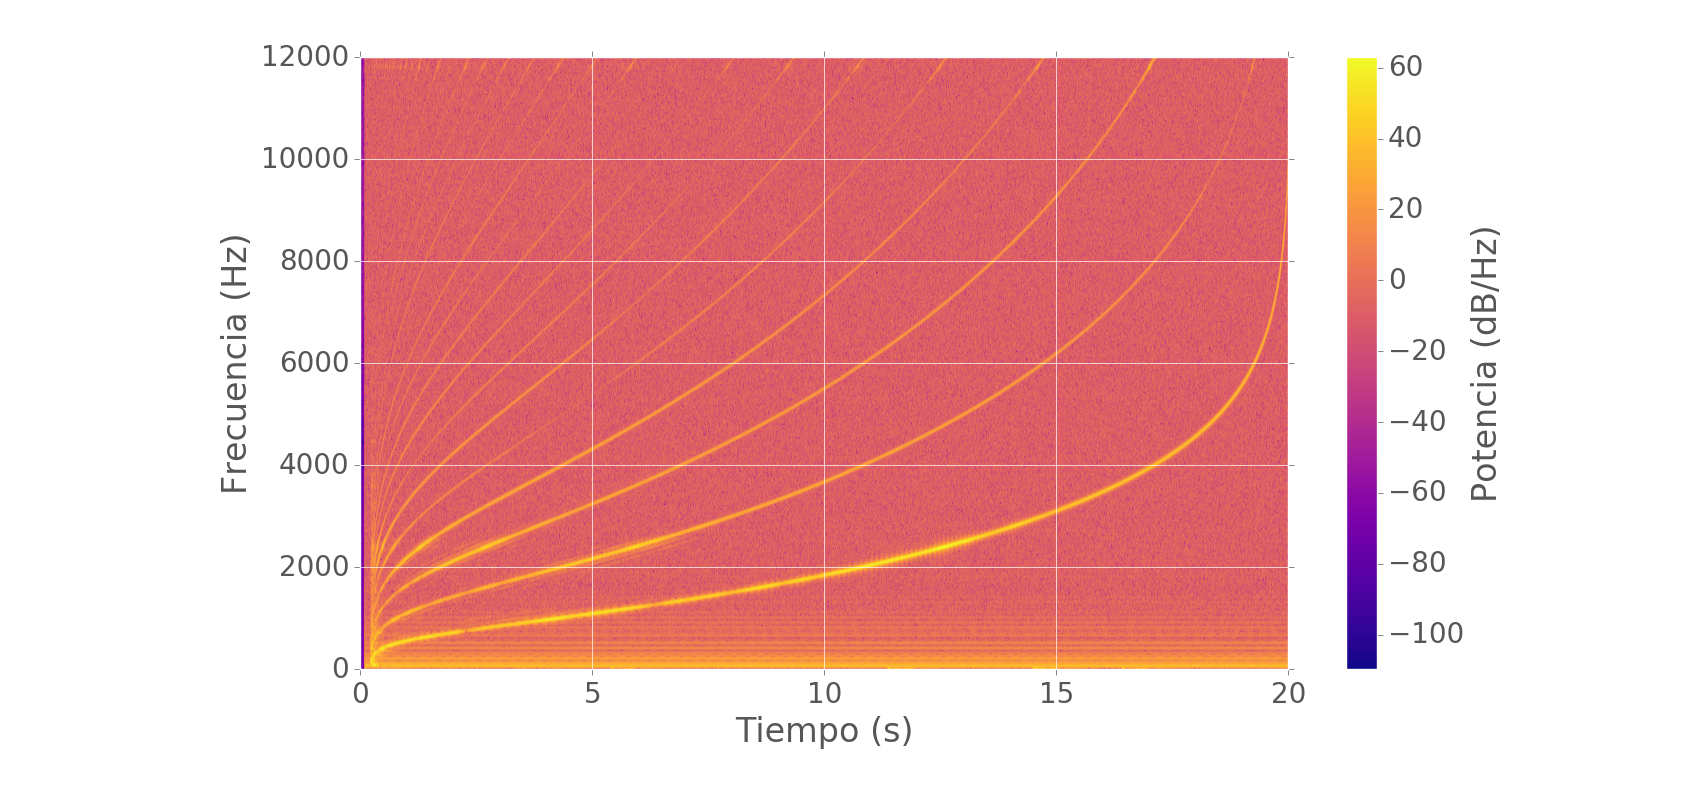
\includegraphics[scale=.43]{testrec.png}
		\caption{Grabación de la señal de prueba en una pecera. Se observan las frecuencias de la señal original y las distorsiones armónicas cuyas frecuencias son múltiplos enteros de las frecuencias originales.}
	\label{fig:testrec}
\end{figure}

El proceso de deconvolución y separación se explica con el siguiente ejemplo: para comprimir una señal de prueba que pase por 100Hz a los 100ms y 200Hz a 200ms el filtro inverso debe tener un retardo de grupo de -100ms a 100Hz y -200ms a 200Hz. Si el sistema analizado presenta armónicos de segundo orden al pasar por 100Hz, estos serán tratados con el retardo de grupo de -200ms, apareciando en la señal convolucionado a tiempo -100ms. Distorsiones de ordenes mayores aparecerán en momentos aún más negativos. La figura \ref{fig:x1y10} muestra la RI obtenida a partir de la deconvolución de la señal grabada en la figura \ref{fig:testrec}. La barra vertical de alta intensidad al comienzo es la RI: todas las frecuencias encendidas a la vez. Los rulos que se observan al costado son efecto de la distorsión armónica demasiado grande y la circularidad de la FFT en el algoritmo de procesado.

\begin{figure}[H]
	\centering
		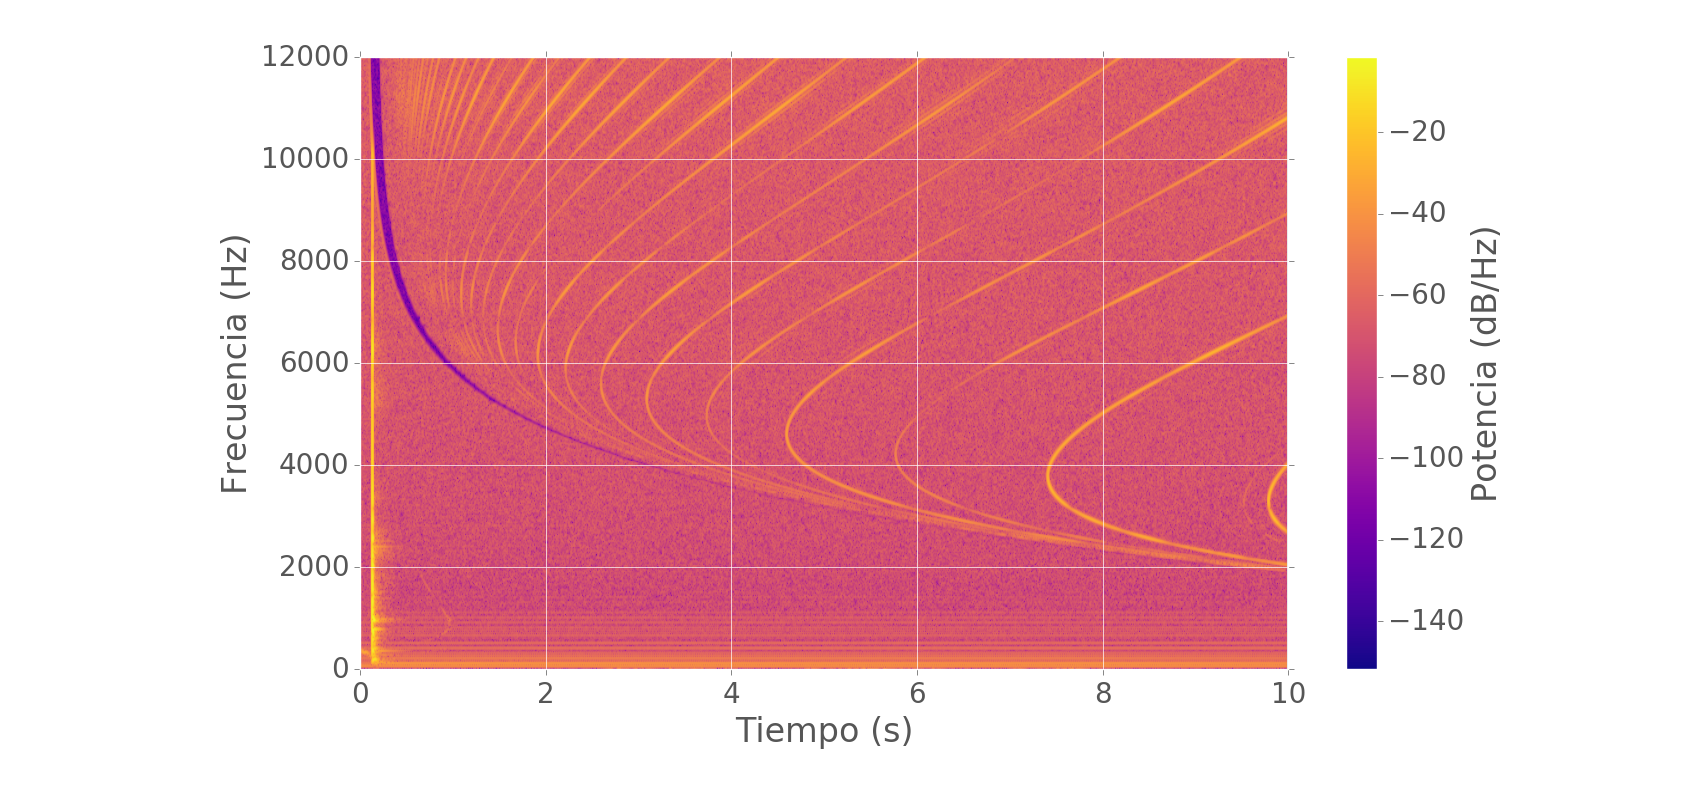
\includegraphics[scale=.43]{x1y10.png}
		\caption{RI de la señal de prueba con distorsión armónica obtenida mediante deconvolución con el filtro inverso.}
	\label{fig:x1y10}
\end{figure}

Los cálculos realizados por COMSOL dan la respuesta (compleja) de la pecera para distintas frecuencias, i.e. una amplitud compleja para cada punto del acuario como respuesta a un forzante armónico de frecuencia única. Realizando los calculos en un rango amplio de frecuencias, se puede obtener (mediante la transformada inversa de Fourier) la respuesta impulso en cada punto de la pecera.

La caracterización y modelado se hizo sobre la pecera con el parlante y luego se realizaron caracterizaciones de la pecera conteniendo una goma de neoprene que sirve de aislante.
\chapter{Desarrollo experimental}
\section{Construcción de la pecera y caracterización}
Se construyó un acuario rectangular utilizando vidrio laminado de 5+5 para la base y 3+3 para las paredes. Las dimensiones totales (internas) son (80x68x15)cm. La profundidad total de agua utilizada para las mediciones es $(12,4\pm0,1)$cm y no fue variada a lo largo del proyecto; el volumen de agua utilizado rondó siempre los 67l. El laminado de 5+5 soporta una columna de 80cm de agua por metro cuadrado, con lo cual la elección del material es por demás segura. El parlante se coloca en un extremo del acuario, en el medio y montado sobre una estructura de goma espuma. En la figura \ref{fig:acuario} se puede observar una fotografía de la pecera cargada con agua y el parlante colocado (sin neoprene). Este desarrollo fué el primer paso realizado en Laboratorio 6.

\begin{figure}[H]
	\centering
		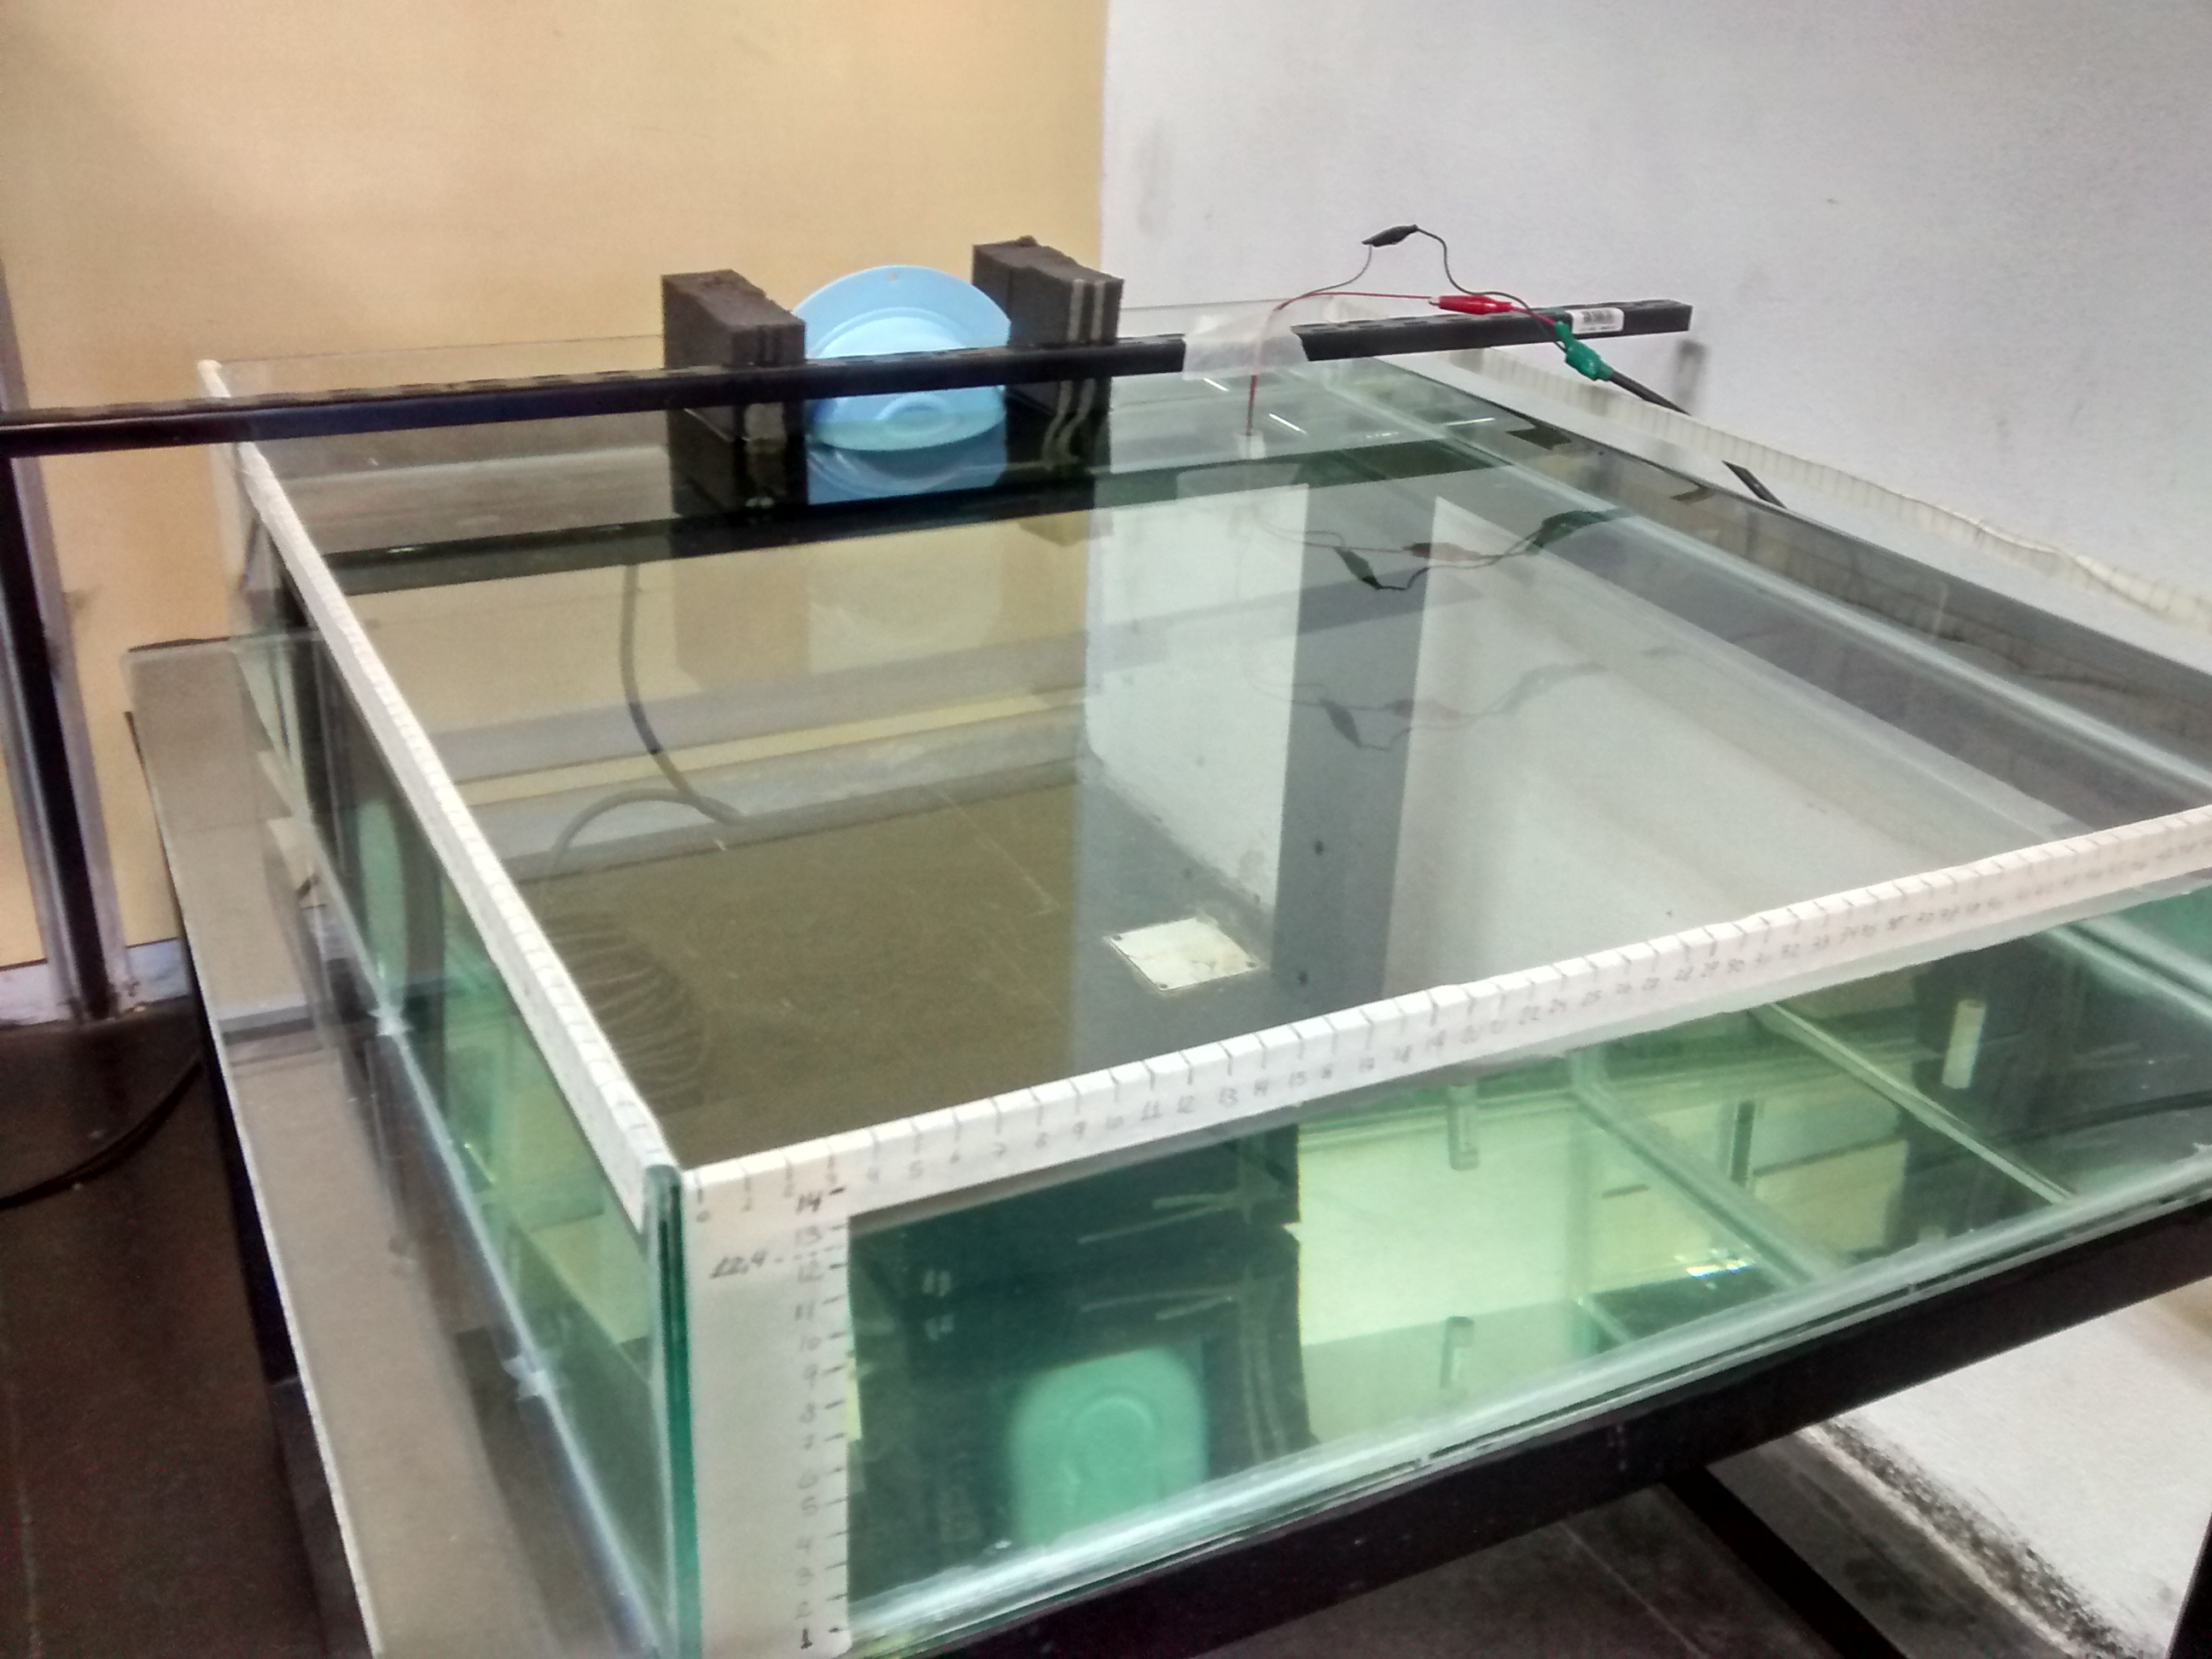
\includegraphics[height=6cm]{pecera.jpg}
		\caption{Fotografía del acuario donde se pueden observar el parlante (celeste) y un hidrófono (montado sobre la barra negra).}
	\label{fig:acuario}
\end{figure}

Para la caracterización se tomó una grilla de puntos en el acuario sobre los cuales se midió la RI mediante el proceso de deconvolución de barridos detallado en la sección \ref{sec:introsweeps}. En la figura \ref{fig:grilla} se muestra un esquema del acuario donde se observan, marcadas en rojo, las posiciones donde se ha caracterizado la RI. La grilla comienza a $(30\pm1)$cm del frente del parlante y avanza cada $(4\pm1)$cm hasta $(62\pm1)$cm respecto del parlante. En la otra dirección, se realizaron 16 mediciones equiespaciadas en $(3,0\pm0,5)$cm, empezando a $(10,0\pm0,5)$cm de una de las paredes.

\begin{figure}[H]
	\centering
		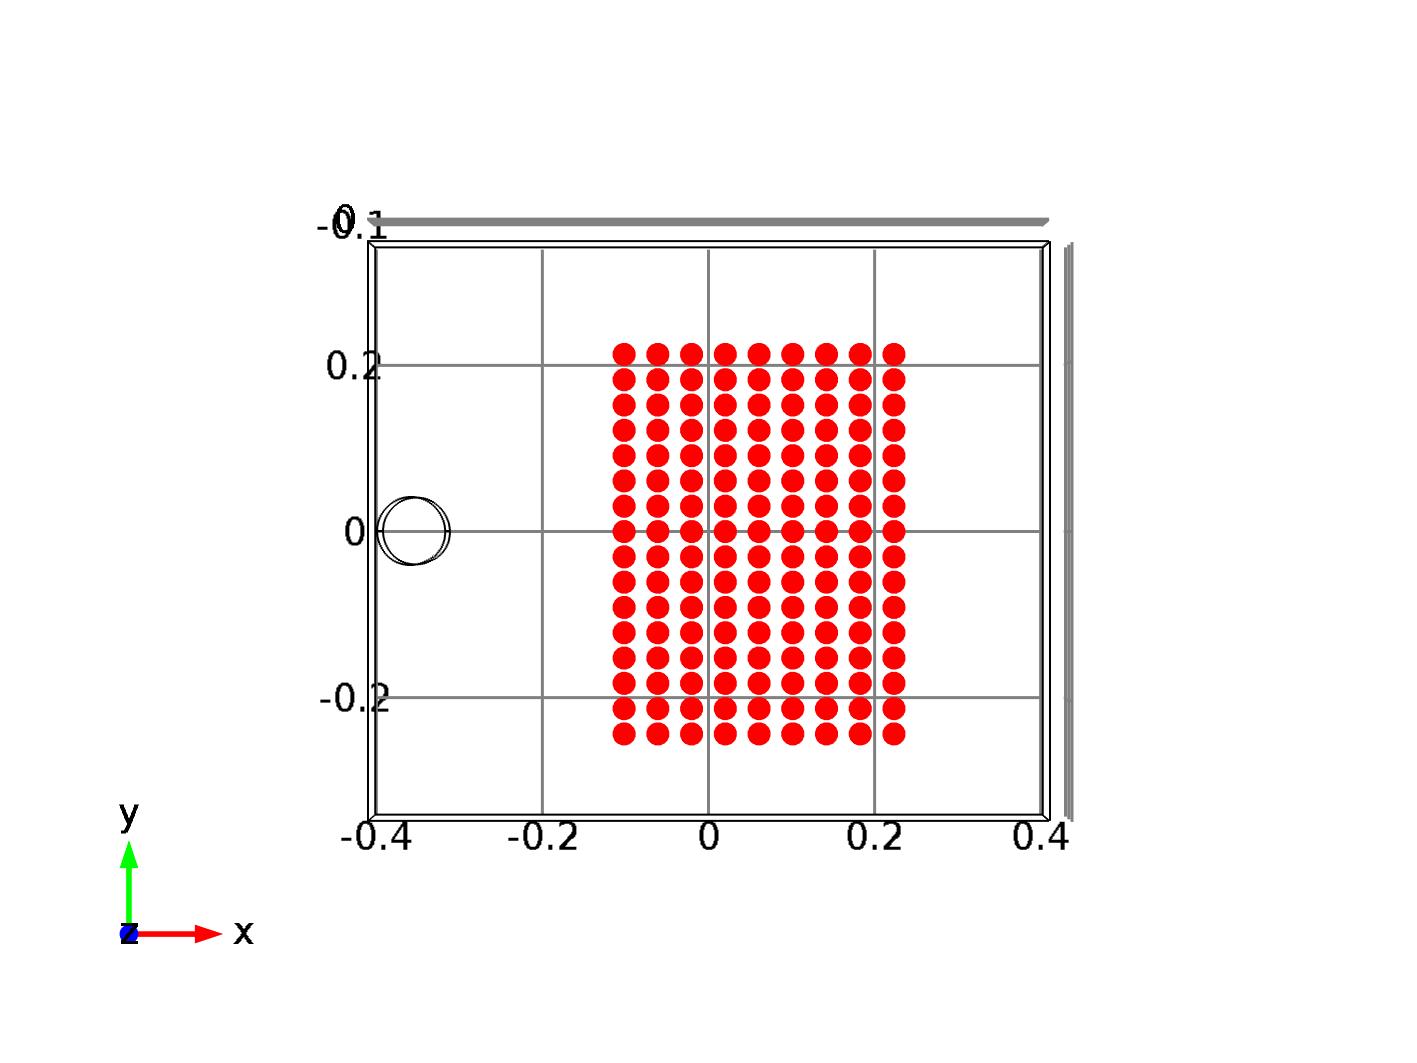
\includegraphics[height=7cm]{puntosmedidos.png}
		\caption{Grilla de puntos donde se caracterizó la RI.}
	\label{fig:grilla}
\end{figure}

El proceso de caracterización consiste entonces en:
\begin{enumerate}
	\item Generar un barrido y su filtro inverso con un script en Matlab. Los scripts fueron desarrollados por Oygo Sound LLC con las ecuaciones de [MullerMassarani] y puede bajarse de [6]. El barrido utilizado dura 20s y comprende un rango de frecuencias desde 400Hz hasta 10kHz. La frecuencia de muestreo es de 48kHz y se mantuvo esa misma frecuencia de muestreo para todas las grabaciones del proyecto (tanto las realizadas en Laboratorio 6 como Laboratorio 7).
	\item El hidrófono (SQ34, Sensor Technology) se conecta a la PC mediante un amplificador diferencial de ganancia 20x.
	\item El parlante se conecta a la PC mediante un amplificador de audio de 8$\Omega$ de impedancia y 30W máximo de salida. La amplificación utilizada para la caracterización fué de alrededor de $\approx$ 22W.
	\item Con el hidrófono en cada una de las posiciones de la grilla, se reproduce y graba en simultáneo el barrido y su respuesta utilizando el programa Audacity. La elección del programa radica en su facilidad de uso y la eficiencia de recursos de la PC para grabar durante todo el día.
	\item Finalmente, se procesa la grabación con el filtro inverso para obtener la respuesta impulso. Un script en Python realiza la convolución mediante transformadas rápidas de Fourier (FFT) y da como resultado las dos partes de la respuesta (lineal y no lineal). El script se encuentra en el apéndice \ref{ap:extractIR}.
\end{enumerate}

Las mediciones se realizaron con la pecera sin neoprene, como en la figura \ref{fig:acuario}, y luego incluyendo al neoprene como se muestra en la figura \ref{fig:conneo}. El neoprene se utilizó como aislante con el objetivo dosminuir la intensidad de los modos normales de la pecera excitados por el parlante.

\begin{figure}[H]
	\centering
		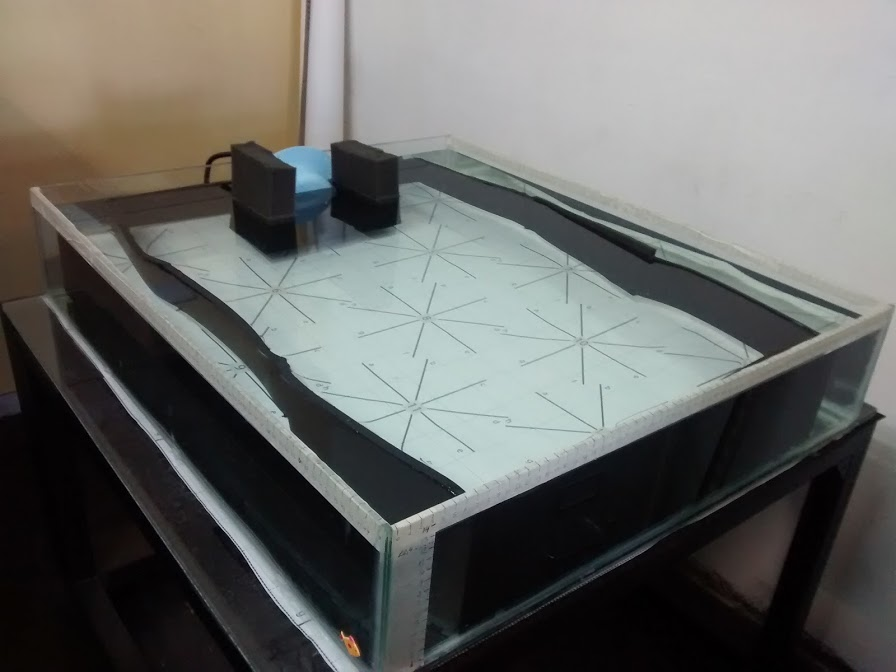
\includegraphics[height=6cm]{con_neoprene.jpg}
		\caption{Configuración con neoprene. La grilla observada debajo de la pecera corresponde a experimentos que no son de este proyecto y no afecta a ninguna de las mediciones realizadas.}
	\label{fig:conneo}
\end{figure}

Todas las caracterizaciones sin neoprene se realizaron durante Laboratorio 6 y el neoprene sólo se utilizó a partir de Laboratorio 7 . Sin embargo, durante el primer mes de Laboratorio 7 se repitieron las mediciones de la RI sin neoprene de las primeras cuatro filas de la grilla. Algún efecto que no se pudo identificar, probablemente sobreamplificación del parlante, no permitía separar la RI de la distorsión armónica.

\paragraph{Comentario sobre calibraciones:}
Todas las mediciones fueron realizadas utilizando una placa de sonido como dispositivo de adquisición. La placa de sonido mapea linealmente la tensión en la entrada de micrófono para que ocupe todo el rango de valores entre -1 y 1 con una resolución de 16 bits. Realizar una única calibración de tensión a valor mostrado en la PC es difícil ya que hay que considerar la ganancia del amplificador del hidrófono y el volumen de la PC, el cual además varía de una PC a otra. Para los estudios realizados esto no significa un problema ya que en todos los casos la variable de interés es la frecuencia medida y sólo interesan amplitudes relativas. Sin embargo, se determinó que para las configuraciones usadas (volumen máximo en PC y ganacia de 20x en el hidrófono), 30mV equivalen al máximo valor de amplitud en la escala de la PC. En lo que resta del informe, todas las amplitudes de sonidos medidas o generadas con la PC se mostrarán en unidades arbitrarias (del intervalo -1 a 1).

\section{Estudios comportamentales}
\subsection{Setup experimental, programa de adquisición y control}
Para los estudios comportamentales se delimitó una zona experimental en la primer mitad de la pecera utilizando el neoprene como se muestra en la figura \ref{fig:conneobis} (la elección se explica en la sección \ref{sec:rescompo} de los resultados y también se caracterizó la RI en esta configuración). El pez puede nadar libremente por la zona experimental y se lo estimula con algún sonido a intervalos de tiempo de 6 o 7 minutos. Un par de electrodos son conectados a un amplificador diferencial de ganancia 20x para medir la DOE y se filma al pez desde arriba con una cámara fotográfica a 40fps.

\begin{figure}[H]
	\centering
		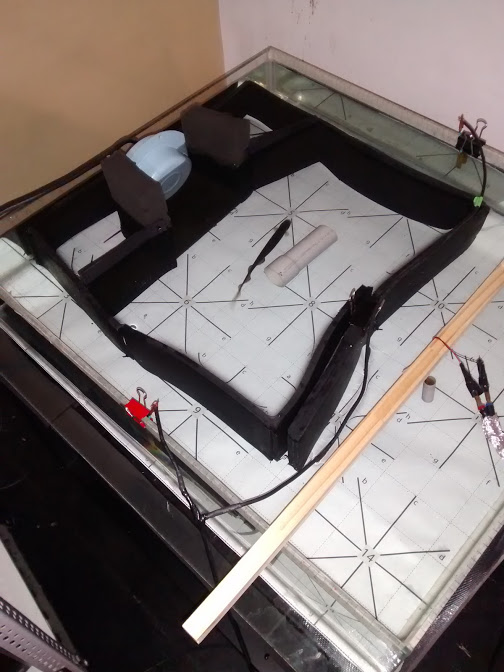
\includegraphics[width=6cm, height=6cm]{con_neo_bis.jpg}
		\caption{Configuración con neoprene utilizada para los estudios comportamentales. Sobre las paredes de la pecera se monta el par de electrodos y sobre la barra de madera el hidrófono y un LED (se enciende al emitir sonidos por el parlante y sirve como referencia visual del comienzo del estímulo en las filmaciones).}
	\label{fig:conneobis}
\end{figure}

La adquisición de datos y todo el control del experimento (salvo la filmación que es manual) se realiza a través de la placa de sonido de una PC mediante un programa escrito en Python 3.5. Utilizando la librería Sound Device y basándose en un ejemplo de su propia documentación [7] se adquiere la señal de la entrada estéreo de micrófono; son dos canales, uno utilizado para el par de electrodos y el otro para el hidrófono. Otro script que utiliza la librería PyAudio permite emitir tonos puros con frecuencia, duración y amplitud programados por el usuario y sonidos desde archivo (.wav). Una mínima interfaz de usuario muestra en un gráfico una ventana temporal de tamaño programable con las mediciones de los dos canales en tiempo real. El programa fué realizado en Laboratorio 7 y se planea su uso para otros experimentos realizados en el LFBM, tanto con peces eléctricos como dorados.

El único aspecto del setup que no fue automatizado es la filmación, ya que la cámara utilizada no cuenta con conexión a PC. Para sincronizar las filmaciones con los experimentos sin depender del volumen grabado por la cámara, se escribió un script para una placa Arduino que enciende un led cada vez que el programa de adquisición y control emite un estímulo. El led queda encendido durante toda la duración del estímulo, permitiendo ver en el video cuándo empieza y termina el sonido.

Todos los programas realizados se encuentran en el apéndice \ref{ap:programapython}.

\subsection{Condiciones de los experimentos}

Utilizando el mismo script de Matlab que genera las señales se prueba se hicieron diez barridos en frecuencia cortos para utilizar como estímulo. Todas las características de estos estímulos se encuentran listadas en la tabla \ref{tab:estimulos} (los barridos son llamados Sweeps). Se utilizaron también tonos puros de amplitud variable a 400Hz y 15ms de duración.

Los estímulos fueron aplicados en orden aleatorio y a intervalos de 6 a 7 minutos para prevenir la habituación del animal. El procedimiento para cada medición consiste en comenzar a grabar (único paso manual), adquirir la DOE durante algunos segundos y luego emitir el sonido con el programa de adquisición y control. La adquisición previa sirve de linea de base y sólo se requieren unos pocos segundos para determinar la frecuencia de descarga antes del estímulo (en ausencia de estimulación la frecuencia de descarga se mantiene constante). Todas las grabaciones se realizaron a 40fps ya que esta estapa de mediciones es exploratoria: sólo se busca saber con qué sonidos se puede gatillar la respuesta de escape o sobresalto y si hay correspondencia motora. En casos donde se requiere analizar la cinemática de la respuesta motora, las grabaciones se deben hacer a 240fps mínimo debido que a que la duración total de la respuesta es de 60ms a 80ms. Esto último no se realizó en este trabajo.

\begin{table}[H]
\centering
\resizebox{\textwidth}{!}{%
\begin{tabular}{c|c|c|c}
\doublerule
Tipo de estímulo        & Duración (ms)        & Frecuencia (Hz)                     & Amplitud (u. a.)         \\	\midrule
\multirow{10}{*}{Sweep} & 10                   & 500-1500                            & \multirow{10}{*}{1}      \\
                        & 15                   & 500-1500                            &                          \\
                        & 20                   & 500-1500                            &                          \\
                        & 25                   & 500-1500                            &                          \\
                        & 10                   & 500-1000                            &                          \\
                        & 15                   & 500-1000                            &                          \\
                        & 20                   & 500-1000                            &                          \\
                        & 25                   & 500-1000                            &                          \\
                        & 10                   & 500-8000                            &                          \\
                        & 15                   & 500-8000                            &                          \\	\midrule
\multirow{10}{*}{Tono}  & \multirow{10}{*}{15} & \multirow{10}{*}{400}               & \multicolumn{1}{c}{0.5}  \\
                        &                      &                                     & \multicolumn{1}{c}{0.55} \\
                        &                      &                                     & \multicolumn{1}{c}{0.6}  \\
                        &                      &                                     & \multicolumn{1}{c}{0.65} \\
                        &                      &                                     & \multicolumn{1}{c}{0.7}  \\
                        &                      &                                     & \multicolumn{1}{c}{0.75} \\
                        &                      &                                     & \multicolumn{1}{c}{0.8}  \\
                        &                      &                                     & \multicolumn{1}{c}{0.85} \\
                        &                      &                                     & \multicolumn{1}{c}{0.9}  \\
                        &                      &                                     & \multicolumn{1}{c}{0.95}	\\ \bottomrule
\end{tabular}%
}
\caption{Tabla de estímulos utilizados.}
\label{tab:estimulos}
\end{table}
\chapter{Resultados y discusión}

\section{Caracterización de la RI sin neoprene} 

\subsection{Comparación entre las mediciones y el modelo COMSOL}

Los modelos realizados en COMSOL muestran la respuesta en frecuencias del acuario en toda su extensión. Para condiciones de borde suaves los primeros modos normales son los debidos al bloque de agua y concuerdan con las primeras frecuencias aproximadas por la ecuación \ref{eq:resonancias}, de $\approx 6200\pm10$Hz con las medidas del acuario. En las figuras \ref{subfig:comsolsuave} y \ref{subfig:comsolmedio} se pueden observar gráficos de la respuesta en frecuencia calculada por COMSOL para un punto de la pecera utilizando las dos condiciones de borde explicadas en la introducción: todos bordes suaves, y condición de impedancia. Para el primer tipo de condiciones de borde sólo se observan modos de frecuencias superiores a 6kHz, mientras que en el segundo se observan algunos de baja intensidad en casi todo el rango estudiado. En todas las simulaciones la presión total de la onda emitida por el parlante es de 1Pa.

\begin{figure}[H]
	\begin{subfigure}[b]{.49\textwidth}
		\centering
			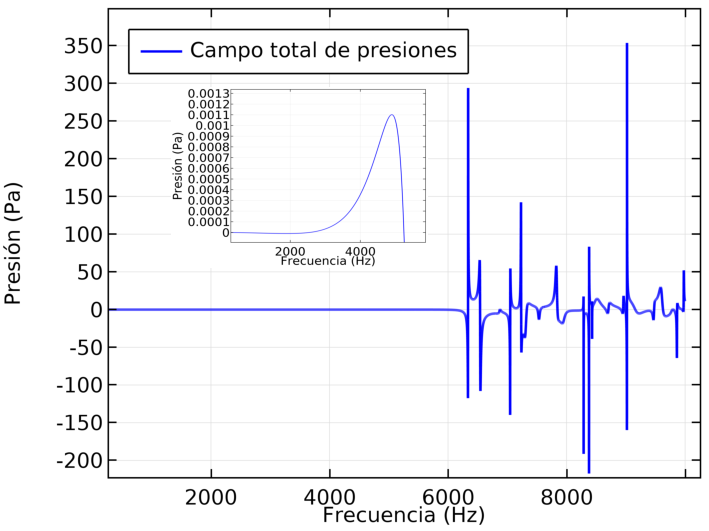
\includegraphics[width=\textwidth, height=4cm]{presiones1.pdf}
			\caption{Bordes suaves.}
			\label{subfig:comsolsuave}
	\end{subfigure}
	\hfill
	\begin{subfigure}[b]{.49\textwidth}
		\centering
			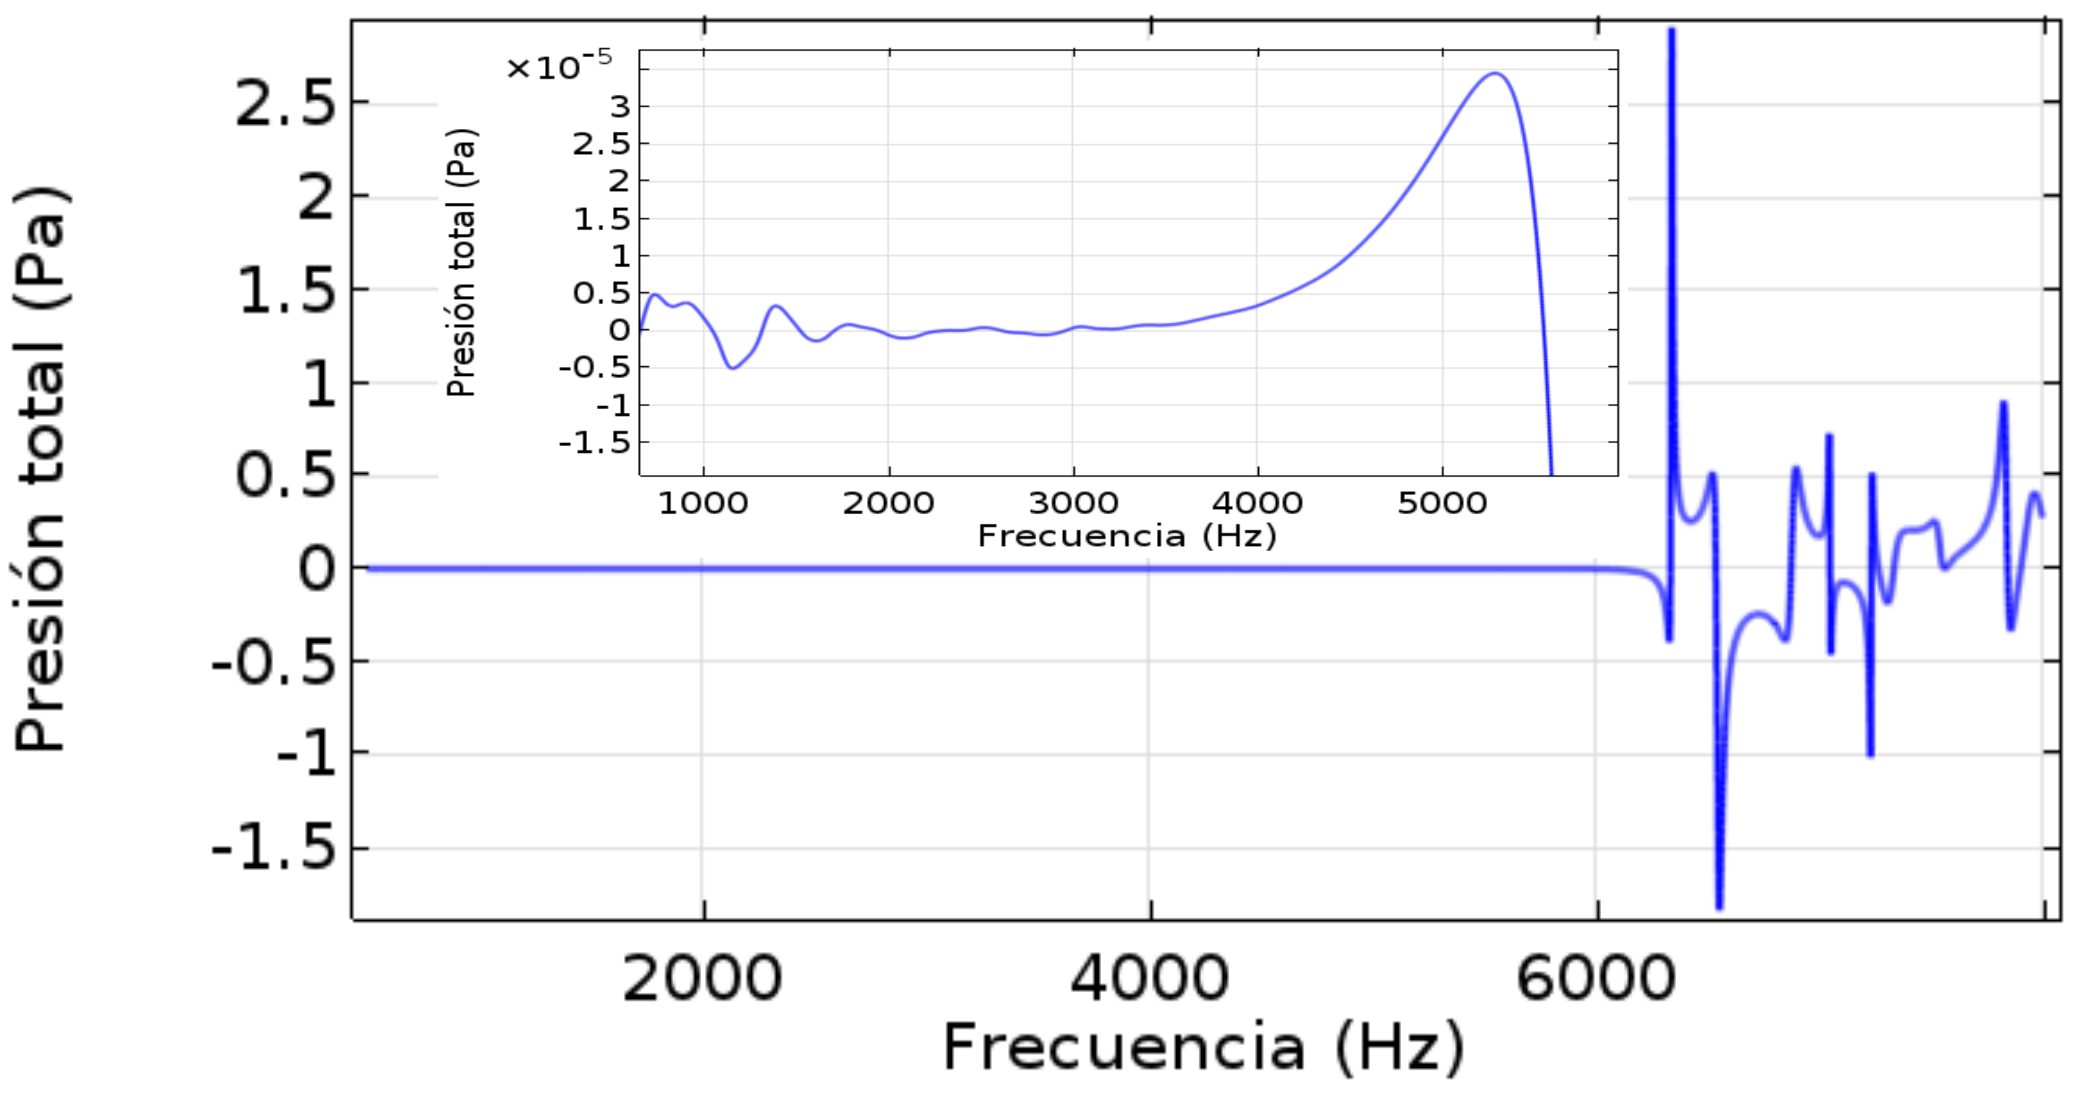
\includegraphics[width=\textwidth, height=4cm]{frcomsol.png}
			\caption{Condición de impedancia.}
			\label{subfig:comsolmedio}
	\end{subfigure}
	\caption{Respuesta en frecuencias del acuario calculada por COMSOL.}
	\label{fig:frcomsol}
\end{figure}

En las RI medidas los modos de alta frecuencia sólo aparecen en la mitad de la pecera más alejada del parlante (el parlante sólo excita esos modos en esa mitad del acuario). En todo el acuario, sin embargo, se observan los modos de bajas frecuencias. En las figuras \ref{subfig:x1y34}, \ref{subfig:x1y34zoom}, \ref{subfig:x7y34} y \ref{subfig:x7y34zoom} se muestran las RIs medidas en distintos puntos de las dos mitades de la pecera. Allí, todos los modos normales se ven como barras horizontales de gran intensidad.

\begin{figure}[H]
		\begin{subfigure}[b]{\textwidth}
			\centering
			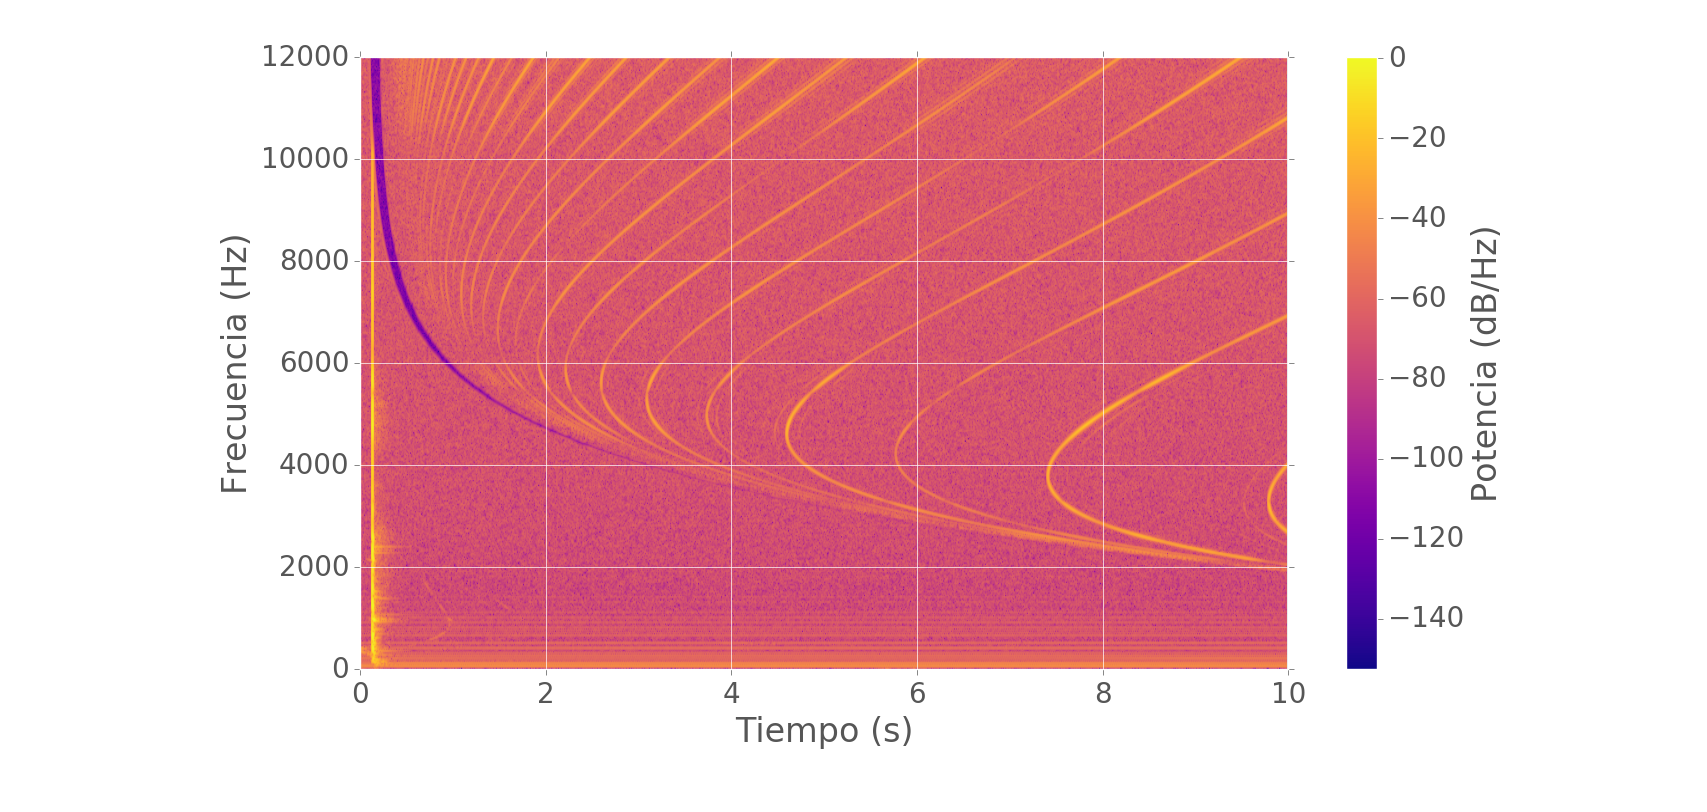
\includegraphics[width=\textwidth]{x1y34.png}
			\caption{RI completa.}
			\label{subfig:x1y34}
		\end{subfigure}

		\begin{subfigure}[b]{\textwidth}
			\centering
			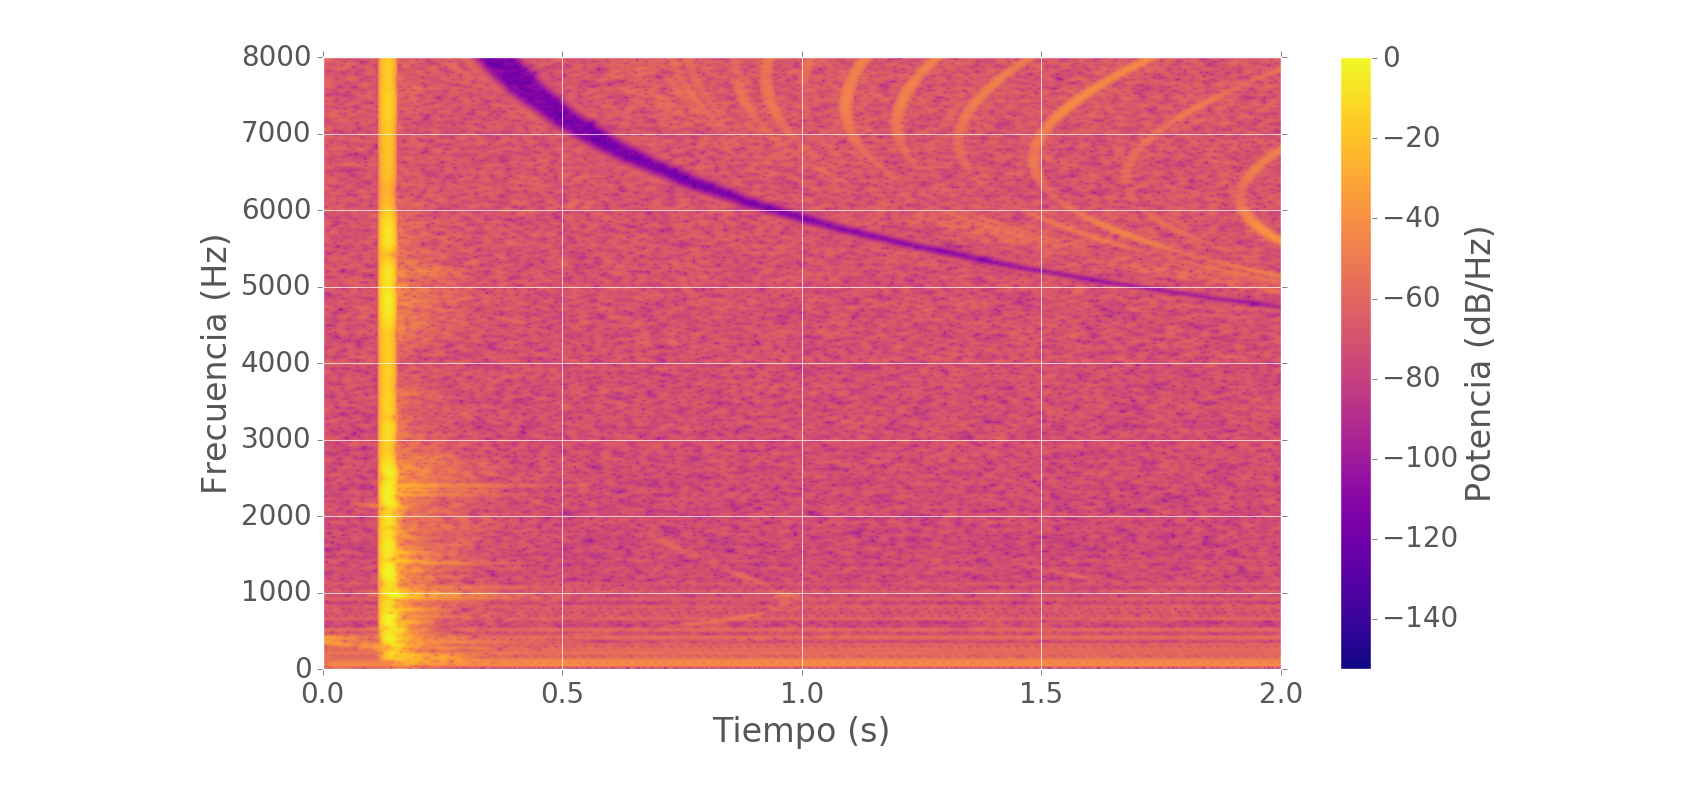
\includegraphics[width=\textwidth]{x1y34zoom.png}
			\caption{Detalle de \ref{subfig:x1y34}.}
			\label{subfig:x1y34zoom}
		\end{subfigure}
		\caption{RI en la primer mitad de la pecera donde se observan los modos de baja frecuencia. Las franjas violetas son artefactos causadas por el método de deconvolución-}
		\label{fig:modosbajos1}
\end{figure}

\begin{figure}[H]
		\begin{subfigure}[b]{\textwidth}
			\centering
			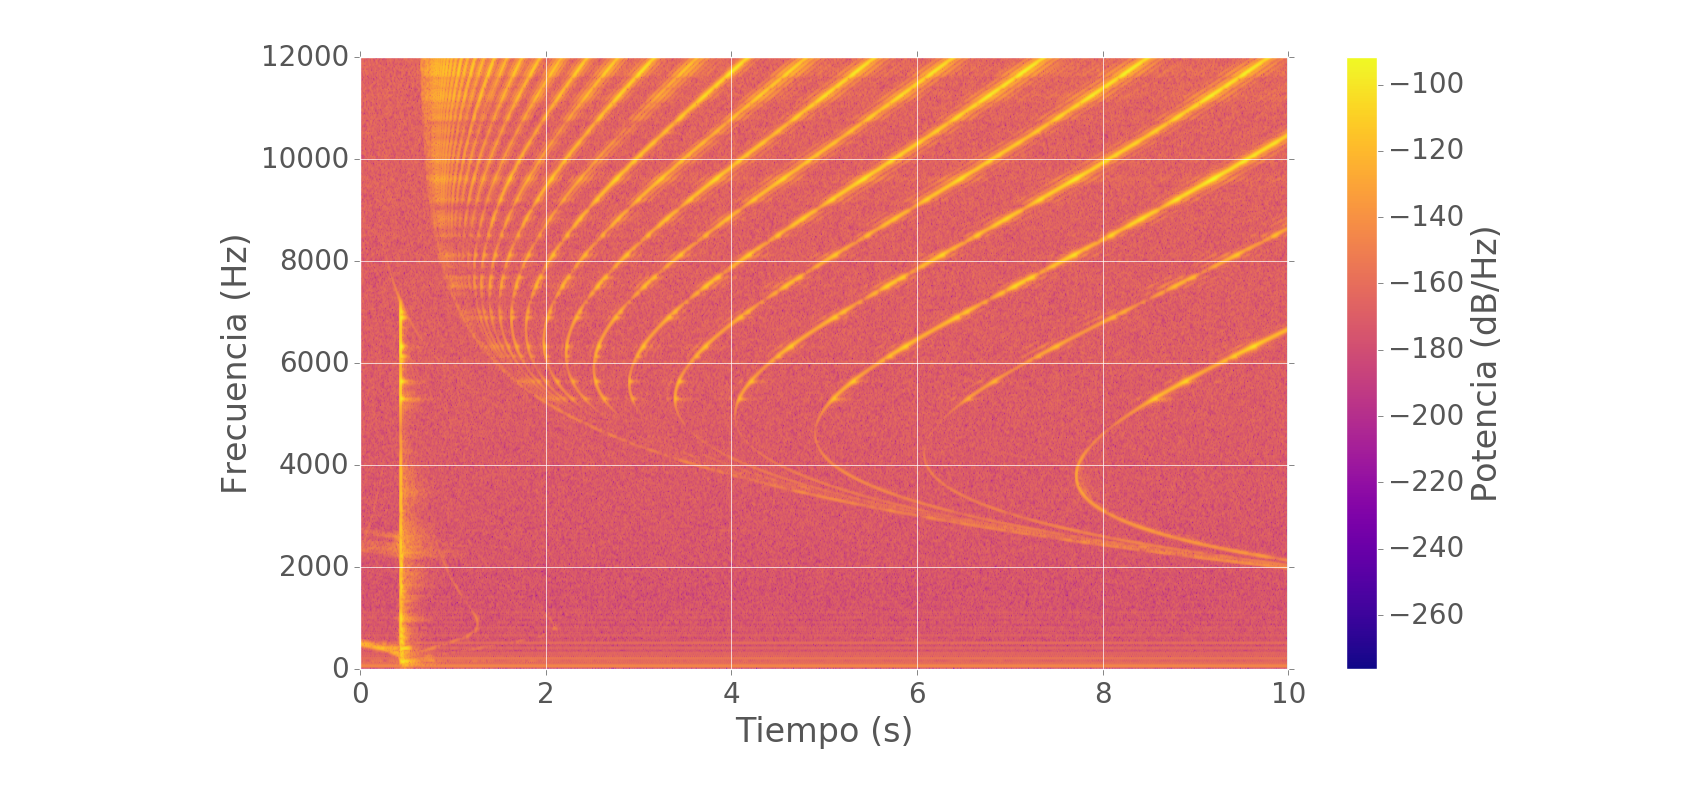
\includegraphics[width=\textwidth]{x7y34.png}
			\caption{RI completa.}
			\label{subfig:x7y34}
		\end{subfigure}

		\begin{subfigure}[b]{\textwidth}
			\centering
			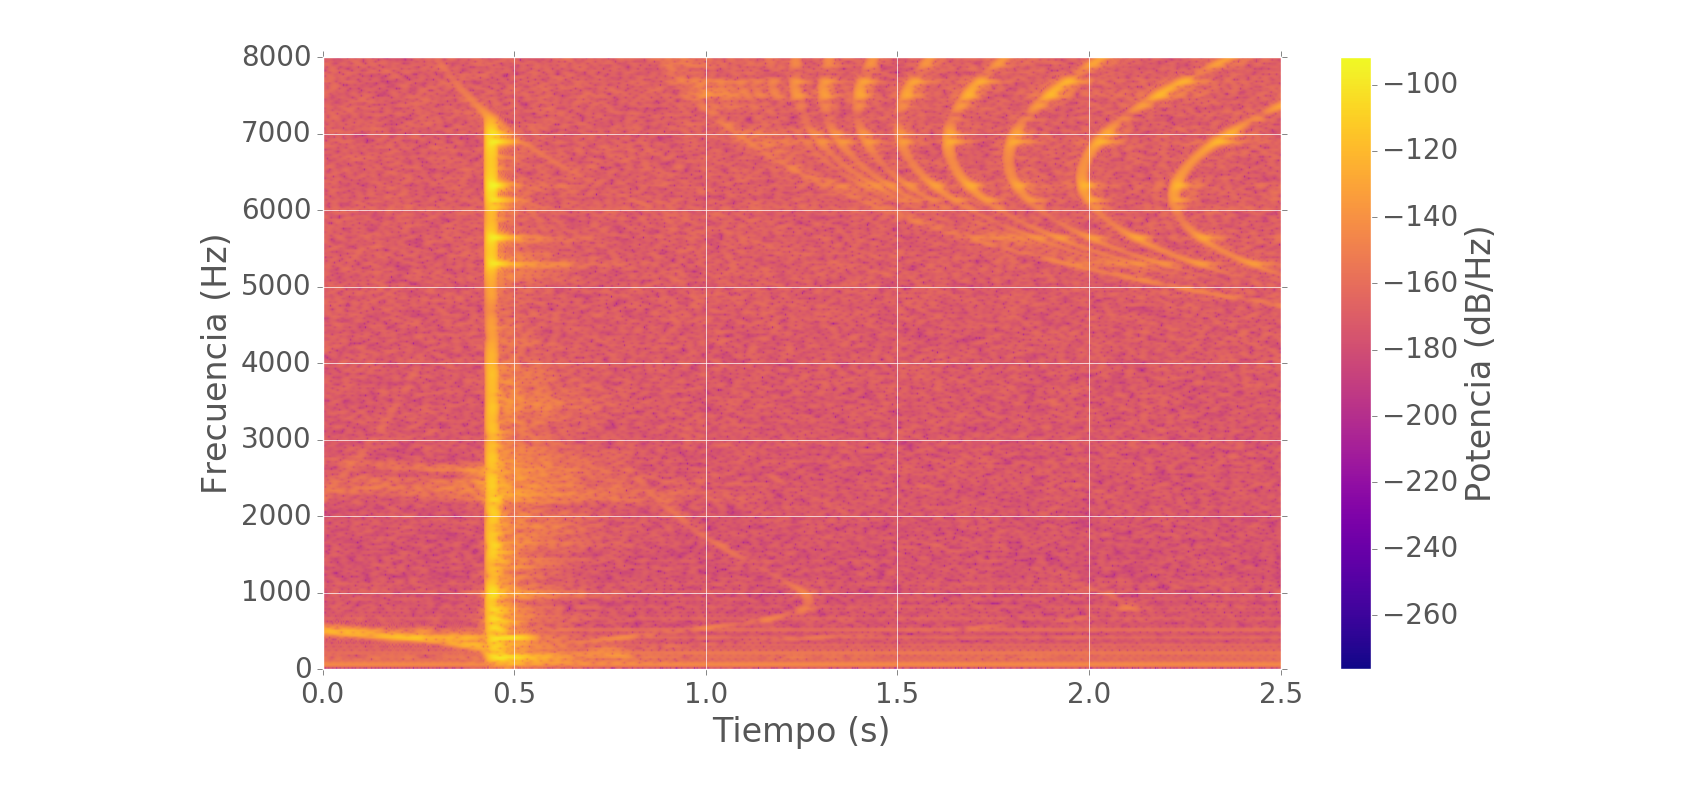
\includegraphics[width=\textwidth]{x7y34zoom.png}
			\caption{Detalle de \ref{subfig:x7y34}.}
			\label{subfig:x7y34zoom}
		\end{subfigure}
		\caption{RI en la segunda mitad de la pecera donde se observan los modos de baja y alta frecuencia.}
		\label{fig:modosaltos1}
\end{figure}

Los resultados obtenidos indican que las condiciones de borde más acordes a la realidad son aquellas en que la superficie libre se modela a partir del cambio de impedancias. En principio, para obtener una predicción completa de todos los campos involucrados es necesario incluir en COMSOL un modelo de emisión del parlante (si bien los modos son propios de la pecera, el parlante puede excitar distintos modos en distintos puntos).

\subsection{Patrones y direccionalidad del campo de presiones}
\label{sec:rescompo}

\begin{figure}[H]
	\begin{subfigure}[b]{.48\textwidth}
		\centering
		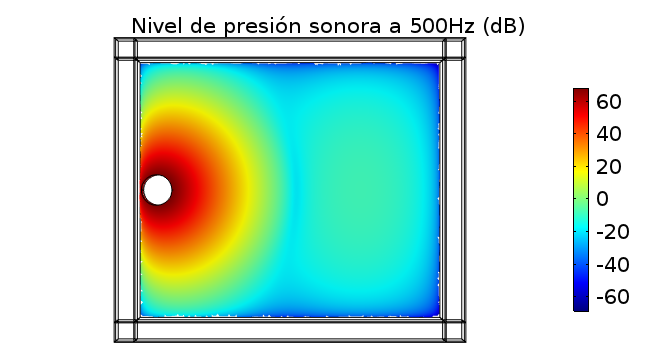
\includegraphics[width=\textwidth , height=4cm]{comsolcampo1.png}
	\end{subfigure}
	\begin{subfigure}[b]{.48\textwidth}
		\centering
		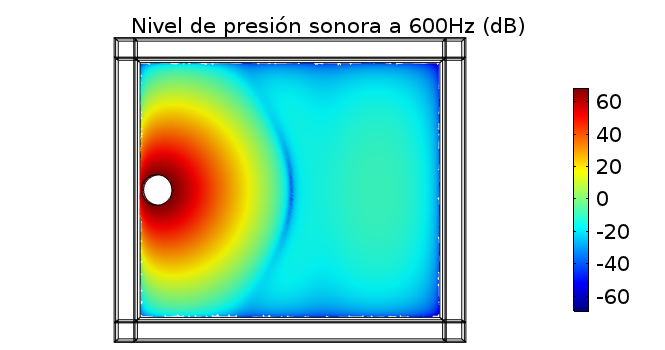
\includegraphics[width=\textwidth , height=4cm]{comsolcampo2.png}
	\end{subfigure}
	
	\begin{subfigure}[b]{.48\textwidth}
		\centering
		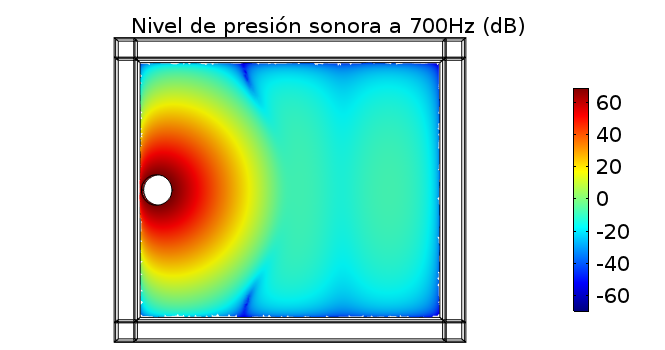
\includegraphics[width=\textwidth , height=4cm]{comsolcampo3.png}
	\end{subfigure}
	\begin{subfigure}[b]{.48\textwidth}
		\centering
		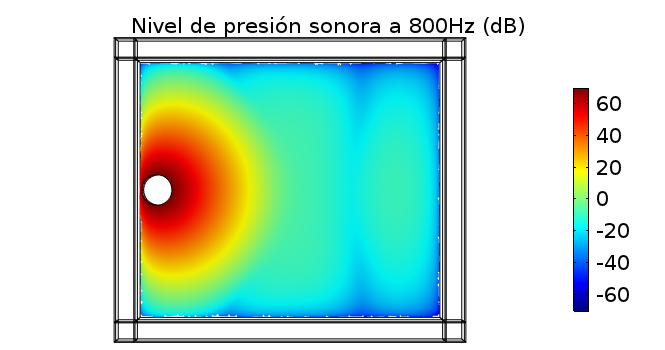
\includegraphics[width=\textwidth , height=4cm]{comsolcampo4.png}
	\end{subfigure}
	
	\begin{subfigure}[b]{.48\textwidth}
		\centering
		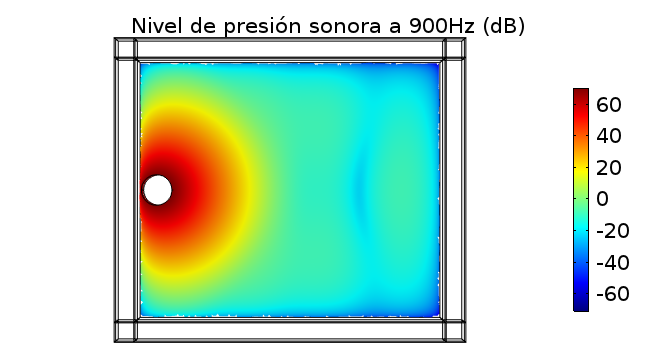
\includegraphics[width=\textwidth , height=4cm]{comsolcampo5.png}
	\end{subfigure}
	\begin{subfigure}[b]{.48\textwidth}
		\centering
		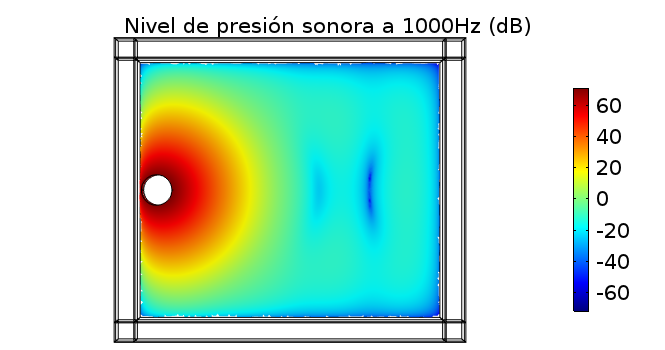
\includegraphics[width=\textwidth , height=4cm]{comsolcampo6.png}
	\end{subfigure}
	
	\begin{subfigure}[b]{.48\textwidth}
		\centering
		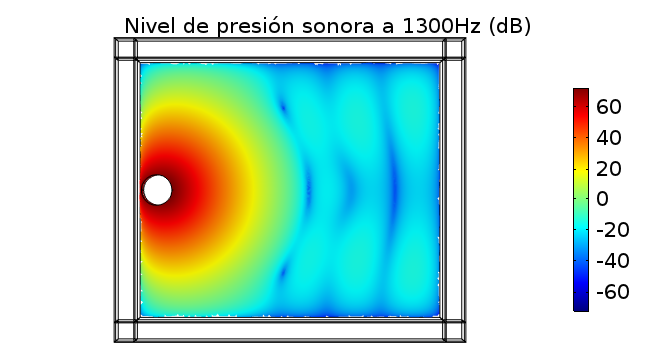
\includegraphics[width=\textwidth , height=4cm]{comsolcampo7.png}
	\end{subfigure}
	\begin{subfigure}[b]{.48\textwidth}
		\centering
		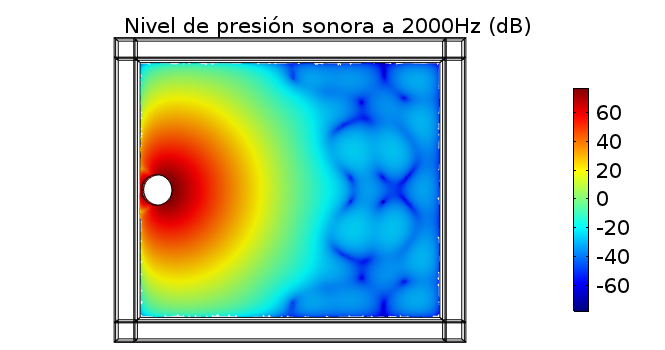
\includegraphics[width=\textwidth , height=4cm]{comsolcampo8.png}
	\end{subfigure}
	\caption{Campos de presiones calculados por COMSOL en toda la pecera.}
	\label{fig:campos}
\end{figure}

Para decidir en qué zonas de la pecera se realizarán los experimentos, es necesario observar en el modelo COMSOL cómo son los patrones del campo de presiones para distintas frecuencias. Los resultados del modelo muestran que en la primer mitad del acuario la direccionalidad del campo de presiones está bien definida para todos los modos y es hemiesférica hacia adelante. En la segunda mitad, los modos de bajas frecuencias forman patrones irregulares donde la direccionalidad no es clara: en esa zona no deberían realizarse experimentos comportamentales, ya que no se puede inferir la direccionalidad del estímulo. La figura \ref{fig:campos} muestra los patrones del campo de presiones a distintas frecuencias.

\section{Caracterización de la RI con neoprene}

A raíz de su uso como aislante en aire y su resistencia al agua, se decidió utilizar neoprene como aislante y delimitador de la zona en la que se realicen los experimentos con animales. Sin embargo la velocidad de propagación del sonido en neoprene es muy cercana a la del agua, y el material es casi invisible en lo que respecta a la acústica a bajas frecuencias. A altas frecuencias, el material podría, a lo sumo, interactuar en forma poroacústica. En las figuras \ref{subfig:neoprene1} y \ref{subfig:neoprene2} se pueden observar dos espectrogramas de la RI medida con neoprene en los mismo puntos de las figuras \ref{fig:modosbajos1} y \ref{fig:modosaltos1}.

\begin{figure}[H]
	\begin{subfigure}[b]{\textwidth}
		\centering
		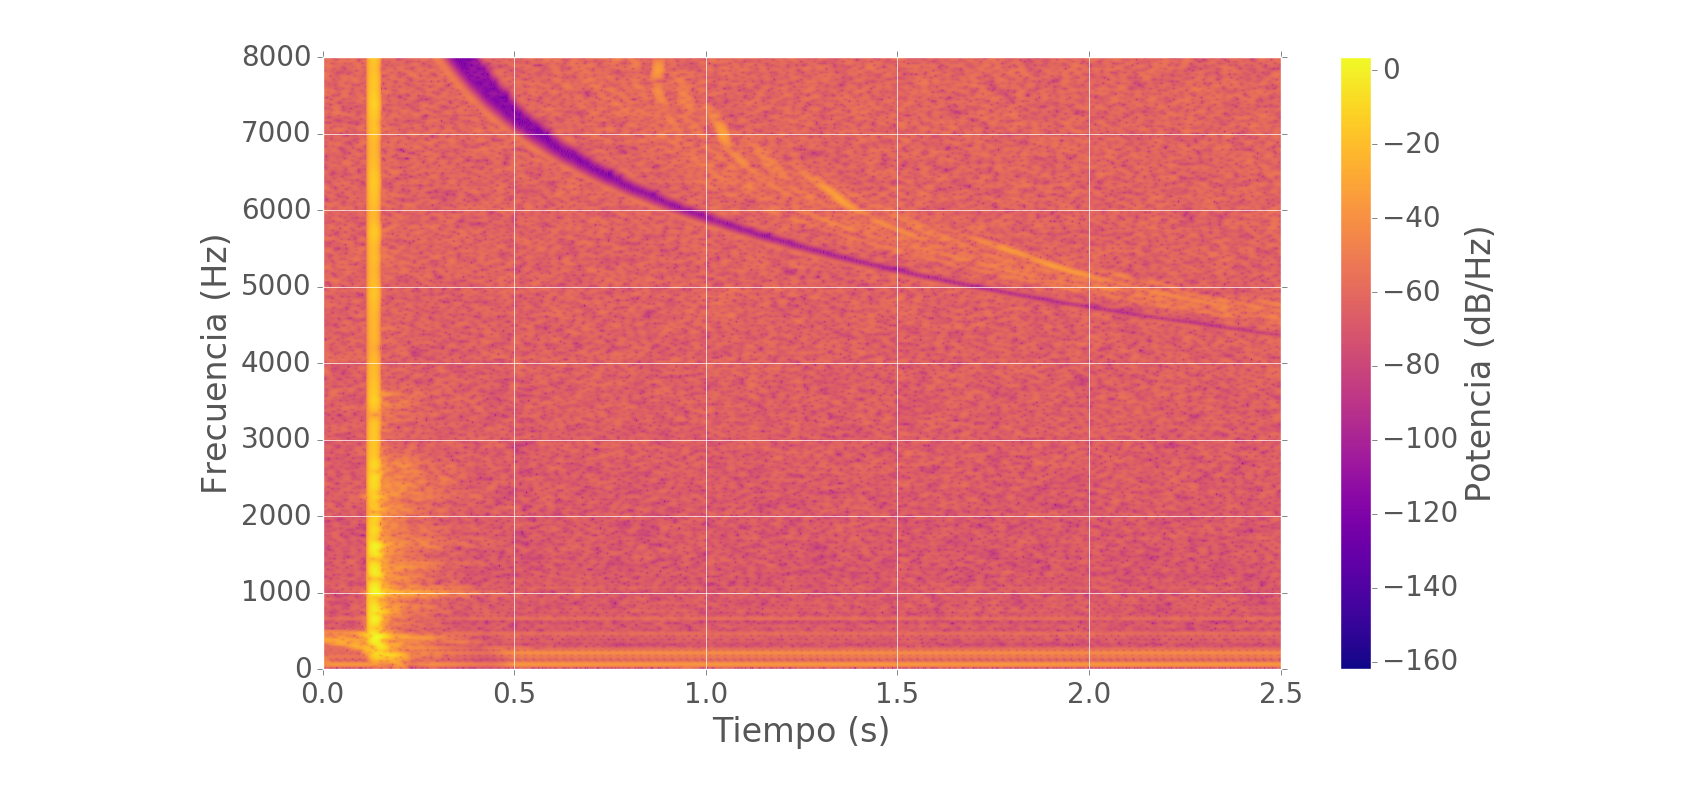
\includegraphics[width=\textwidth , height=6cm]{x1y34neo.png}
		\caption{Primera mitad de la pecera.}
		\label{subfig:neoprene1}
	\end{subfigure}

	\begin{subfigure}[b]{\textwidth}
		\centering
		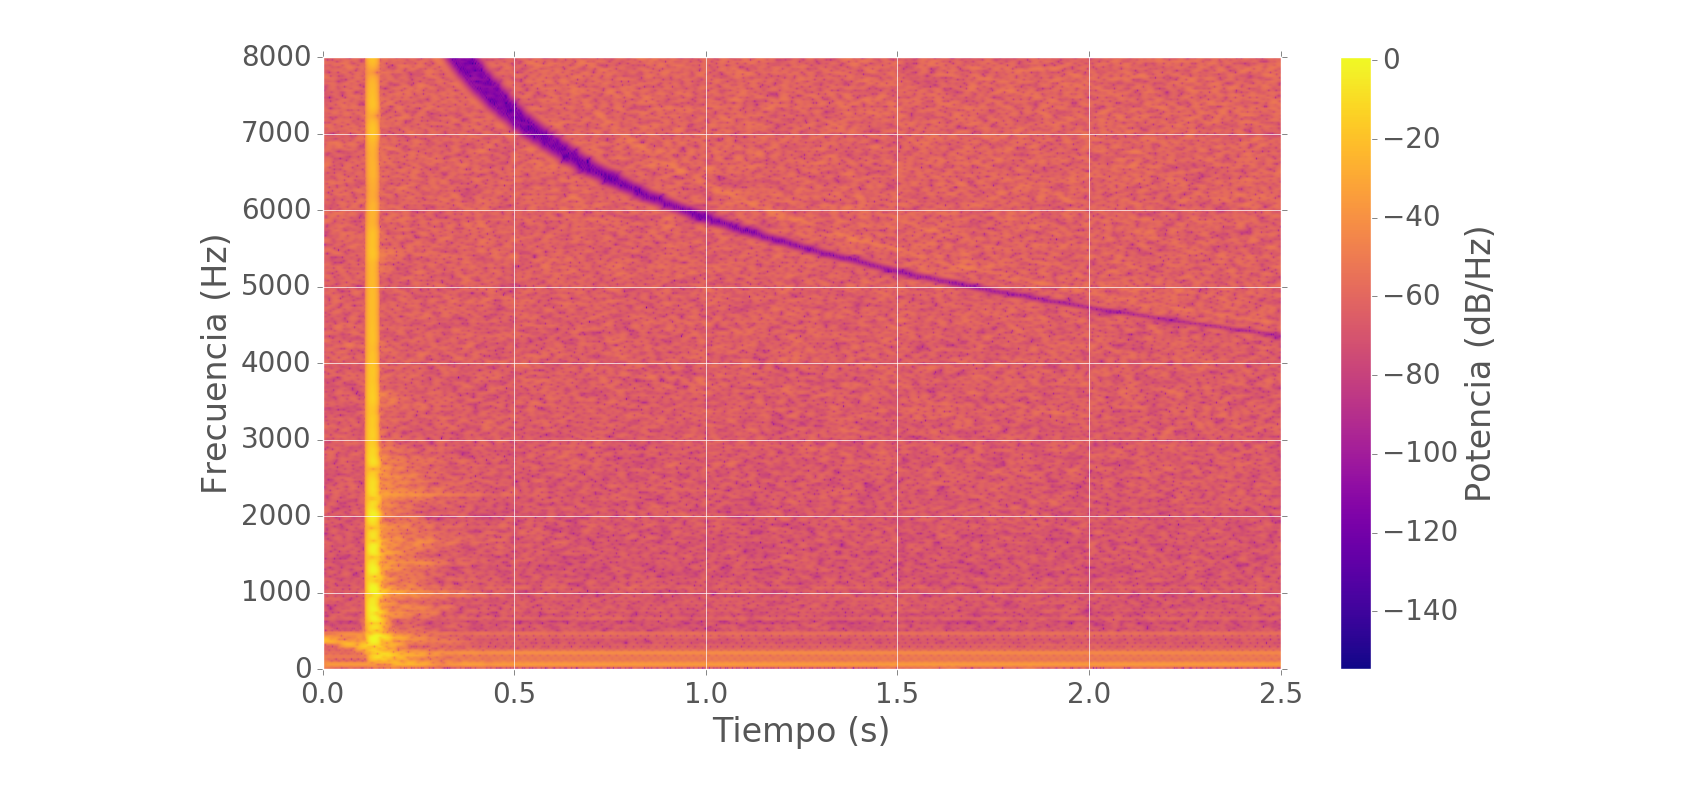
\includegraphics[width=\textwidth , height=6cm]{x7y34neo.png}
		\caption{Segunda mitad de la pecera.}
		\label{subfig:neoprene2}
	\end{subfigure}
	\caption{RI medida con neoprene. Las franjas violetas son artefactos causados por el método de deconvolución.}
\end{figure}

Se realizaron mediciones adicionales utilizando en la configuración de la figura \ref{fig:conneobis}. Esta última configuración fué utilizada para delimitar como zona experimental a la primer mitad del acuario, en la cual se realizaron lo estudios comportamentales. Al no observar cambios cualitativos apreciables en la RI salvo una baja en la intensidad de los modos excitados, se decidió no modelar sus propiedades en COMSOL. Esto puede hacerse si se miden propiedades del material (coeficientes de absorción, módulo de Young, etc.) y se programa al material en COMSOL, ya que el mismo no tiene goma de neoprene en ninguna de sus librerías. 

\section{Experimentos comportamentales}

Con la zona experimental delimitada por el neoprene, se realizaron experimentos comportamentales utilizando los estímulos de la tabla \ref{tab:estimulos}. Tanto para barridos como tonos puros, se observa siempre un aumento en la frecuencia de descarga de la DOE (i. e. disminuye el tiempo entre descargas). La figura \ref{fig:doemiedo} muestra gráficos del tiempo entre descargas y de la DOE misma en función del tiempo de medición.

\begin{figure}[H]
	\centering
		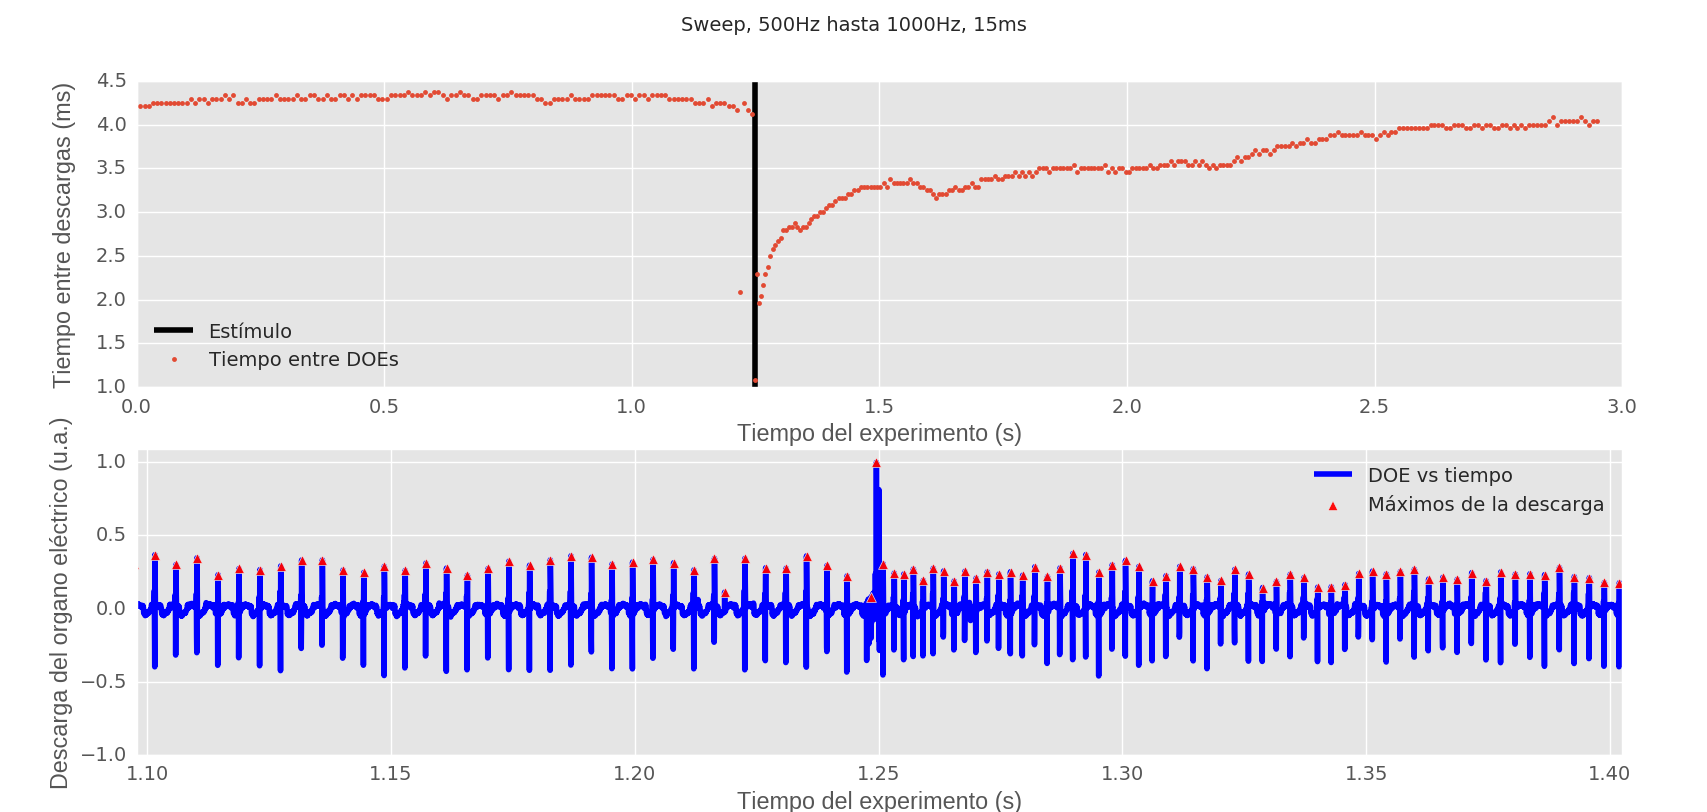
\includegraphics[width=\textwidth]{sw6.png}
	\caption{DOE y tiempo entre descargas. Cada pico marcado con un triángulo rojo es una descarga. Los errores de medición se han tomado como el promedio del ancho mitad de la DOE y son del orden de 0,2ms. El tiempo entre descargas se calcula restando los tiempos entre picos adyacentes.}
	\label{fig:doemiedo}
\end{figure}

En las tablas \ref{tab:rescompo} se muestran los resultados obtenidos con cada estímulo. Se han tenido en cuenta el cambio de tiempo entre descargas al momento del estímulo, $\Delta DOE$, y el tiempo que tarda el animal en volver a su frecuencia basal (tiempo entre descargas antes del estímulo), $\Delta_b$. Si bien el número de mediciones realizadas no permite realizar estadística en cuanto a qué tipo de estímulo es mejor, si se pueden obtener algunos datos útiles:
\begin{itemize}
	\item En todos los casos, el tiempo que tarda el animal en volver a la frecuencia basal es por lo menos dos ordenes de magnitud mayor que la duración del estímulo (y el tiempo entre descargas).
	\item A priori la única diferencia observable a simple vista es que los barridos producen cambios más grandes en la frecuencia de la DOE y tiempos más largos en volver a la frecuencia basal.
\end{itemize}
\newpage
\begin{table}[H]
\centering
%\resizebox{\textwidth}{!}{%
\begin{tabular}{c|c|c}
\doublerule
Estímulo & $\Delta DOE$ (ms) & $\Delta_b$ (s) \\	\midrule
Sweep 1  & 2.2               & 1.1            \\
Sweep 2  & 0.8               & 1.5            \\
Sweep 3  & 1.5               & 1.7            \\
Sweep 4  & 0.4               & 1.4            \\
Sweep 5  & 0.8               & 1.1            \\
Sweep 6  & 2.4               & 2.7            \\
Sweep 7  & 0.6               & 2.3            \\
Sweep 8  & 1.7               & 0.4            \\
Sweep 9  & 0.9               & 2.0            \\
Sweep 10 & 0.4               & 1.0            \\	\midrule
Tono 1   & 0.9              & 1.8            \\
Tono 2   & 0.9               & 1.5            \\
Tono 3   & 0.3               & 0.1            \\
Tono 4   & 0.8               & 0.7            \\
Tono 5   & 1.6               & 0.9            \\
Tono 6   & 0.8               & 0.6            \\
Tono 7   & 1.4               & 1.0            \\
Tono 8   & 1.7               & 1.0            \\
Tono 9   & 0.9               & 0.9            \\
Tono 10  & 0.5               & 0.8            \\	\bottomrule 
\end{tabular}%
%}
\caption{Resultado obtenidos para cada estímulo. Se muestran las disminuciones en los tiempos entre descargas y el tiempo que tarda el animal en volver a la frecuencia basal.}
\label{tab:rescompo}
\end{table}

\chapter{Conclusiones}

Los principales objetivos planteados en el plan de trabajo han sido cumplidos: la caracterización de la pecera para estudios comportamentales permitió demarcar una zona en la cual realizar los experimentos. Las principales complicaciones provinieron de distintas obras y cortes de luz en los laboratorios de la Facultad y de los altos costos de equipos como el acelerómetro.

Las mediciones de la RI permiten saber en qué zonas de la pecera se excitan modos normales y los modelos numéricos cómo son dichos modos. Los resultados obtenidos para bajas frecuencias obligan a la elección de una condición de impedancia por sobre la de bordes suaves en la superficie libre. Los modelos realizados co ndicha condición muestran un buen grado de acuerdo con las mediciones realizadas. Al utilizar la aproximación de bordes suaves en todas las superficies el acuario se comporta como una guía de ondas con sus primeros modos por arriba de 6kHz, todos presentes en las mediciones, pero no se predicen los modos de baja frecuencia.

La inclusión del neoprene mostró eliminar todos los modos de alta frecuencia y disminuir la intensidad de los modos más bajos. A futuro sería interesante y útil elaborar algún método que permita también eliminar los modos de bajas frecuencias y así tener una respuesta plana en toda la pecera y a todas las frecuencias de interés.

En cuanto a los desarrollos puramente técnicos se ha avanzado en la automatización de los experimentos del laboratorio. El programa de adquisición y control realizado se utilizará tanto en estudios de peces eléctricos como dorados y puede ser modificado y ampliado sin dificultades mayores según se requiera en el futuro.
\begin{thebibliography}{10}

\bibitem[1]{kinsler}
    Kinsler, L.E., Frey, A.R., Coppens, A.B. y Sanders, J.V. (2000) Fundamentals of acoustics. Fourth edition. John Wiley; New York.

\bibitem[2]{okumura}
    TSUYOSHI OKUMURA , TOMONARI AKAMATSU y
HONG Y. YAN (2002) ANALYSES OF SMALL TANK ACOUSTICS: EMPIRICAL
AND THEORETICAL APPROACHES, Bioacoustics: The International
Journal of Animal Sound and its Recording, 12:2-3, 330-332.

\bibitem[3]{rogers}
    Rogers et. al. “The Effects of Noise on Aquatic Life II”, A.N. Popper, A.Hawkins (eds.), ch. 115, 933—940.

\bibitem[4]{muller}
    S. Müller, P. Massarani – “Transfer-Function
Measurement with Sweeps”, JAES Vol. 49,
Number 6 pp. 443 (2001).

\bibitem[5]{farina}
     A.Farina – “Advancements in impulse response
measurements by sine sweeps”, 122nd AES Convention, May 2007.

\bibitem[6]{synthsweep}
	\url{https://www.mathworks.com/matlabcentral/fileexchange/29187-swept-sine-analysis}

\bibitem[7]{sounddevice}
	\url{http://python-sounddevice.readthedocs.io/en/0.3.5/examples.html}

\end{thebibliography}
\appendix
\chapter{Programa de adquisición y control para estudios comportamentales}
\label{ap:programapython}

El programa está íntegramente escrito en Python 3.5 y utiliza las librerías Sound Device y PyAudio para grabar y emitir sonidos respectivamente. Cabe aclarar que se puede ``grabar'' cualquier señal analógica de frecuencia superior a 20Hz con una amplitud pico a pico de alrededor de 200mV a 1V. Al no ser datos requeridos por los consumidores, los fabricantes rara vez los listan en las hojas de datos. Por ese motivo, es recomendable aumentar el valor pico a pico de tensión de la señal a medir hasta observar que la PC satura (el efecto se lo llama \emph{clipping}) la señal.

Este programa se utilizó para grabar en estéreo las señales del par de electrodos y la del hidrófono. La segunda sirve como una ``estampa temporal'', permite discernir en qué momento se emitió el estímulo.

Para terminar, utilizando distintas teclas del teclado uno puede abrir archivos de texto en los cuales se guardarán las mediciones y emitir sonidos desde un archivo (un .wav) o tonos puros de frecuencia, amplitud y duración programada por el usuario en el momento.

\section{Programa principal}
\lstinputlisting[language=Python]{chapters/code/experiment.py}
\section{Reproductor de sonidos}
\lstinputlisting[language=Python]{chapters/code/ToneGenerator.py}
\section{Controlador Arduino}
\lstinputlisting[language=Python]{chapters/code/arduino.py}

\chapter{Procesado de grabaciones}
\label{ap:extractIR}

El siguiente script en Python permite obtener la RI de una grabación de la señal de prueba. La función extractIR() toma argumentos un array de NumPy donde esté guardada la grabación y otro con el filtro inverso. Esta función puede importarse hacia otros scripts o Notebooks de Jupyter.

\lstinputlisting[language=Python]{chapters/code/extractIR.py}

\end{document}